\chapter{Event selection}
The event selection has been optimized to get phase space which has more signal compared to the background.
The detail of the whole event selection for 2-lepton channel is shown in this chapter. The event selection in other 0/1-lepton channel is summarized in the appendices.

%overview
First the preselection cuts are applied including basic event cleaning and the trigger requirements, then the specific event selection is applied to the each 0,1,2-lepton channels.
For the main event selection, first the selection of the one $W/Z$ boson decaying leptonically is selected. 
The events are categorized into two regions depends on the type of the jets included. The events has one or more large-R jets are categorized as merged category, otherwise resolved category.  
Then in each channel, the forward jets and the hadronically decaying boson is selected and the Signal region (SR) and the Control region (CR) is defined separately in merged category and resolved category. Finally the selection to enhance the VBS topology is applied before using the machine learning approach to get the final discriminant. The SRs are the regions optimized to maximize the significance of the signal over background, and the CRs are region which is the specifical background-dominant, used for constraining the backgrounds. 
\section{Preselection}
Firstly some pre-selection on the Triggers, event cleaning selections are applied to get the available events and to reject the problematic events. The same selection is applied both for data and MC samples.
The selections with respect to the number of jets and leptons at minimum is applied, as summarized in Table~\ref{tab:presel_CxAOD}.
\begin{table}[H]
\begin{center}
\resizebox{0.55\textwidth}{!}{
\begin{tabular}{|l|c|}
\hline\hline
\multicolumn{2}{|c|}{ Common } \\
\hline\hline
Trigger & listed in Table~\ref{tab:triggers} \\
\hline
Event Cleaning & listed in Section~\ref{subsec:event_cleaning} \\
\hline
Number of jets & $N_j \geq 2$ or $N_J^{\textrm{LCTopo}} \geq 1$ \\
\hline\hline\hline
%\multicolumn{2}{|c|}{ 1-lepton channel } \\
%\hline
%Number of Tight leptons   & $=1$ \\
%\hline
%Number of additional Loose leptons   & $=0$ \\
%\hline
%\ptlv                     & $>75\,\GeV$ \\
%\hline\hline
\multicolumn{2}{|c|}{ 2-lepton channel } \\
\hline\hline
Number of Loose leptons   & $=2$ \\
\hline
The leading lepton \pt    & $> 25$~GeV \\
\hline\hline
%\multicolumn{2}{|c|}{ 0-lepton channel } \\
%\hline\hline
%Number of Loose leptons   & $= 0$ \\
%\hline
%\met                      & $> 140\,\GeV$ \\
%\hline\hline
\end{tabular}
}
\end{center}
\caption{List of the pre-selections applied.
%Definitions of Tight and Loose leptons are found in Sections~\ref{subsec:electron_selection}--\ref{subsec:muon_selection}.
%$N_j$ is the number of signal- and VBF-jets defined in Section~\ref{subsec:jet_selection}.
%$N_J^{\textrm{LCTopo}}$ is the number of large-R jets with $\pt>200\,\GeV$ and $\left| \eta \right| < 2.5$.
} \label{tab:presel_CxAOD}
\end{table}

\section{Leptonically decaying Boson}
The selection of the $W/Z$ boson decaying leptonically is applied before categorizing of the signal region (SR) and the control region (CR).
In 2-lepton channel, the $Z\rightarrow ll $ candidates are identified by requiring two isolated same-flavour leptons. Both leptons are required to be $p_T > 27$GeV.
Opposite charges are required for the muon pairs, not for electrons due to their higher mis-identification rate because of the conversions of photons from bremsstrahlung, especially at high $E_T$. The dilepton invariant mass $m_ll$ is required to be close to the Z boson mass.
For electrons, mass window is required as:
\begin{equation}
83<m_{e e}<99 ~\mathrm{GeV}
\end{equation}
while for muons, the $p_{T,ll}$-dependent mass window is required:
\begin{equation}
\left(85.6-0.0117 p_{\mathrm{T}, \ell \ell}\right)<m_{\mu \mu}<\left(94.0+0.0185 p_{\mathrm{T}, \ell \ell}\right) ~\mathrm{GeV}
\end{equation}
This $p_T,ll$ requirement,which is optimized from the analysis of 2015+16 \cite{} is adopted because of the effect of dimuon mass resolution degradation at high-$p_{T,ll}$.
Data and MC distributions of relevant lepton distribution at the early stage of the selection are shown in Figure~\ref{fig:2lepLeptons}.
\begin{figure}[H]
    \centering
    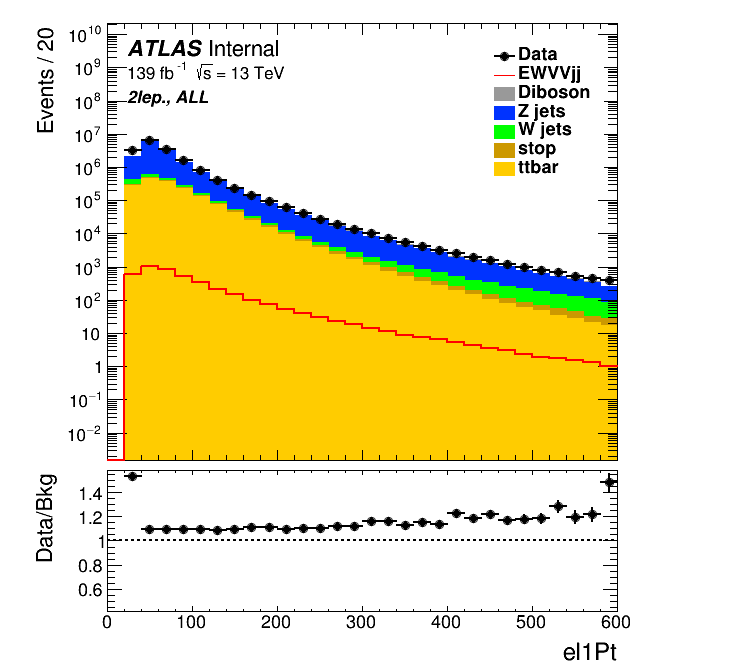
\includegraphics[width=0.4\textwidth]{figures/2lep/dataMC/C_0ptag1pfat0pjet_0ptv_ALL_el1Pt_Log}
    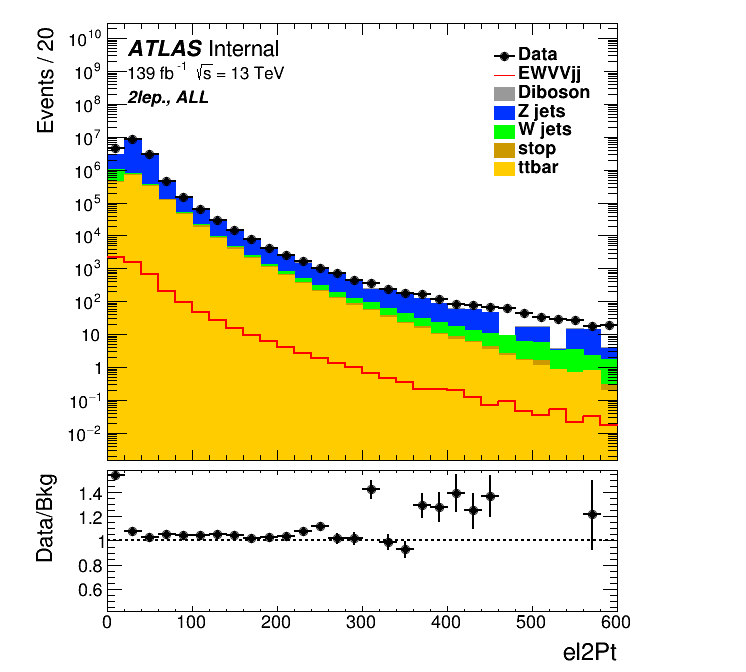
\includegraphics[width=0.4\textwidth]{figures/2lep/dataMC/C_0ptag1pfat0pjet_0ptv_ALL_el2Pt_Log} 
    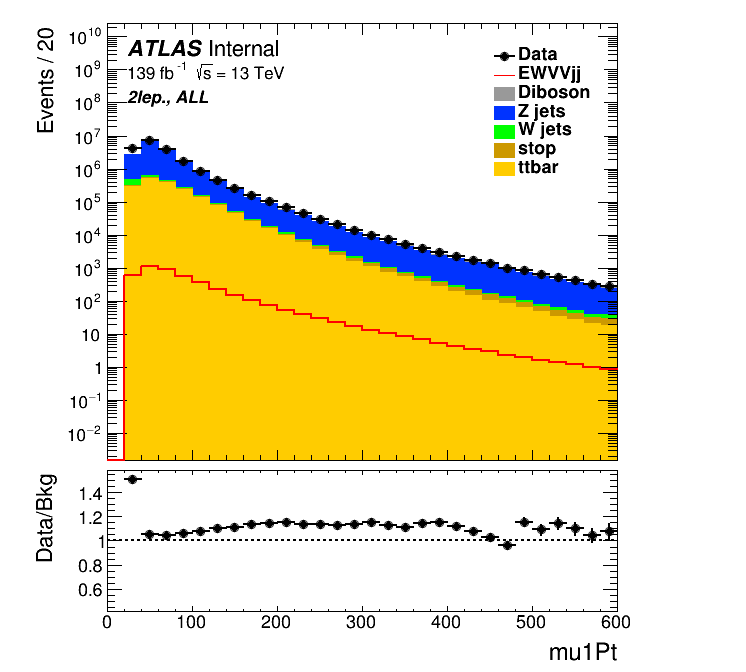
\includegraphics[width=0.4\textwidth]{figures/2lep/dataMC/C_0ptag1pfat0pjet_0ptv_ALL_mu1Pt_Log}
    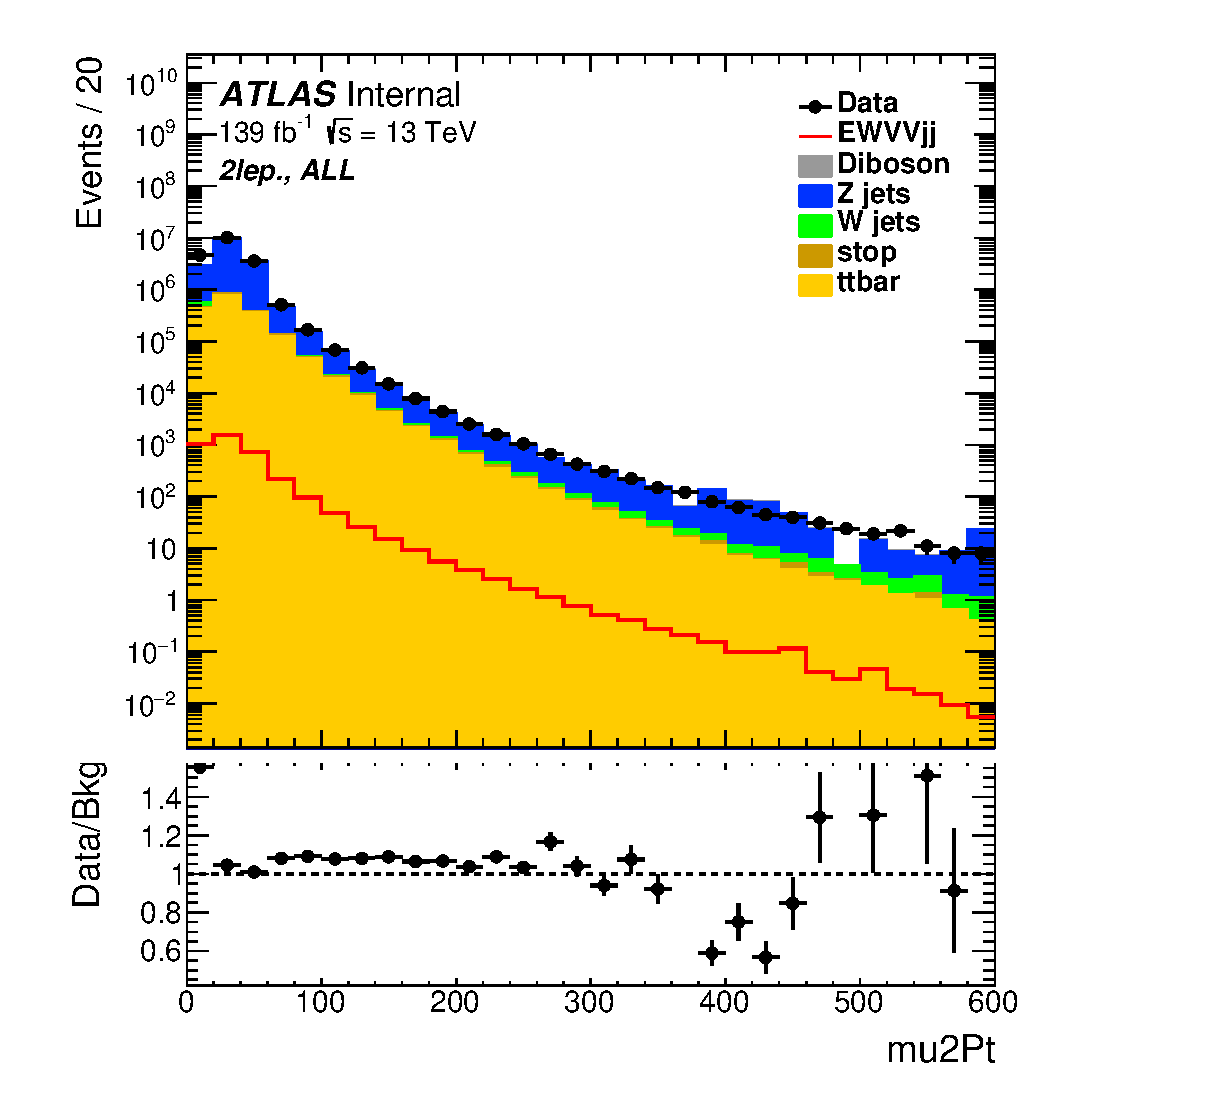
\includegraphics[width=0.4\textwidth]{figures/2lep/dataMC/C_0ptag1pfat0pjet_0ptv_ALL_mu2Pt_Log} 
    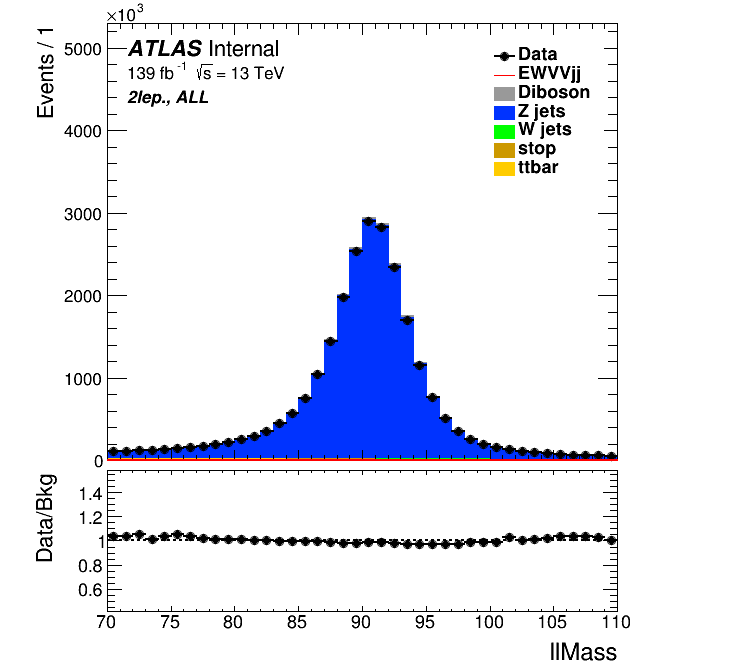
\includegraphics[width=0.4\textwidth]{figures/2lep/dataMC/C_0ptag1pfat0pjet_0ptv_ALL_llMass_Lin}
    \caption{Lepton distributions in 2-lepton channel. The events before any selections are shown. Z mass peak can be seen in $M_{ll}$ distribution.}
    \label{fig:2lepLeptons}
\end{figure}

\section{VBS topology selection}
The VBS event requires to have a pair of small-R jets as a candidate of the forward jets, referred as tagging jets.
The hadronically decaying W/Z boson is reconstructed as either two small-R jets of one large-R jets, which referred as signal jets. The Signal region (SR) and the Control region(CR) is set by requiring these signal jets.

The selection strategy is to first select tagging jets and then select signal jets in order to select the production topology first and then move to the identification of the objects for the decay part of the process.

The tagging jets are required to be b-vetoed to suppress the contribution of the diagrams with $Wtb$ vertex in the electroweak VVjj signals. The fJVT selection to pass the Loose fJVT working point is applied to the small-R jets to suppress the pileup jets contributions.
Tagging jets pair is selected from the oppsite hemisphere, $\eta_{\operatorname{tag} j_{1}} \cdot \eta_{\operatorname{tag} j_{2}}<0$, and to have the highest dijet invariant mass according to its topological features.
Selected tagging jets are required to be $p_T > 30$GeV, and the dijet invariant mass ($m^{tag}_{jj}$) is required to be $m^{tag}_{jj} > 400$GeV.
Figure~\ref{fig:Mtagjj} shows the $m^{tag}_{jj}$ distribution before selecting the SR or CR. 
\begin{figure}[ht]
    \centering
    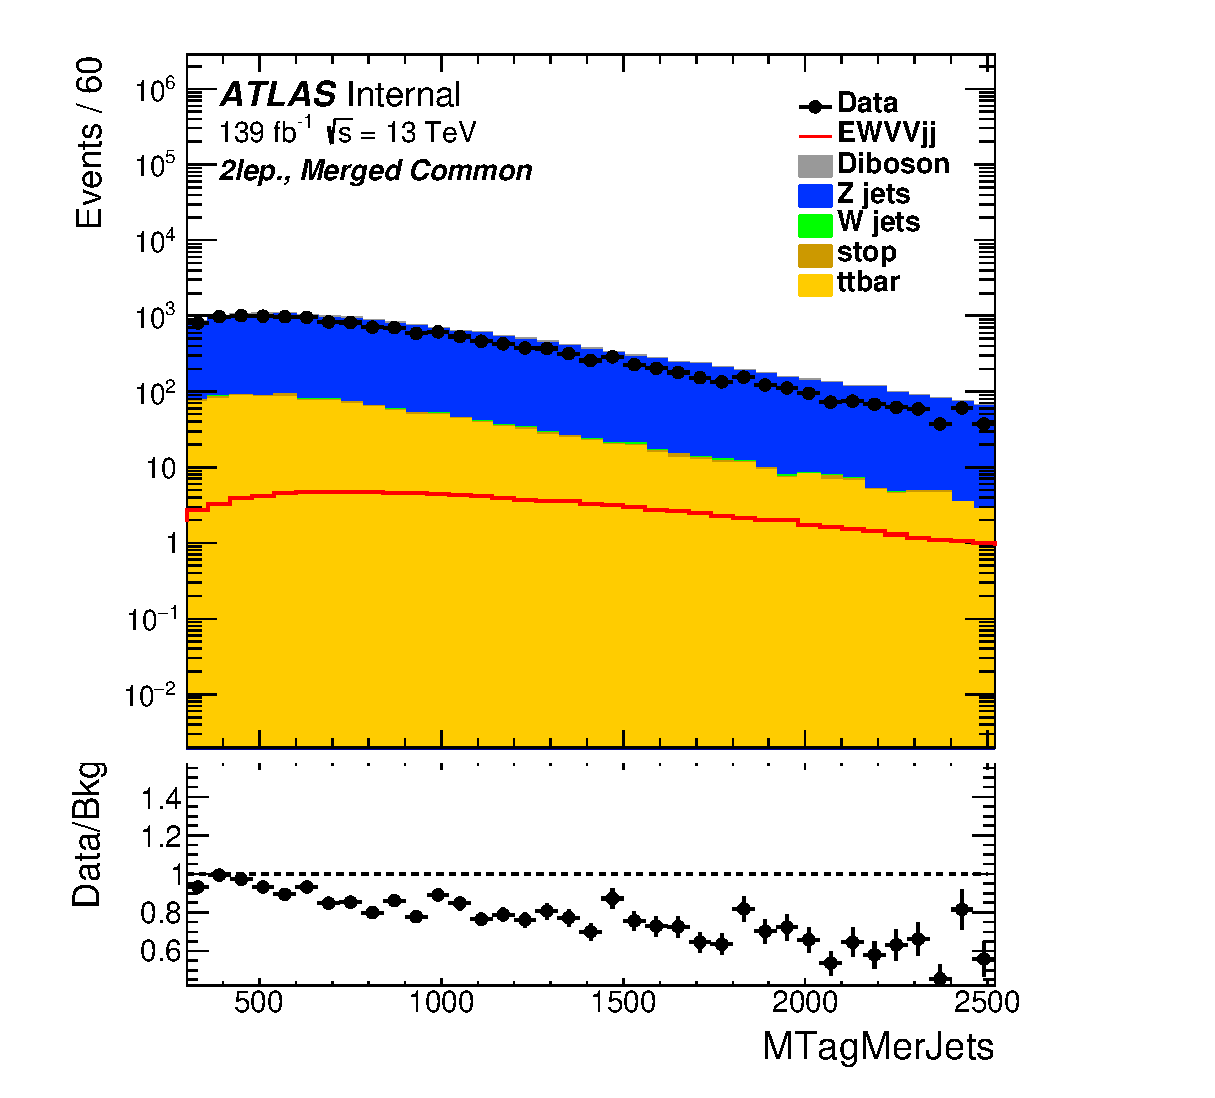
\includegraphics[width=0.4\textwidth]{figures/2lep/dataMC/C_0ptag1pfat0pjet_0ptv_MergedCommon_MTagMerJets_Log}
    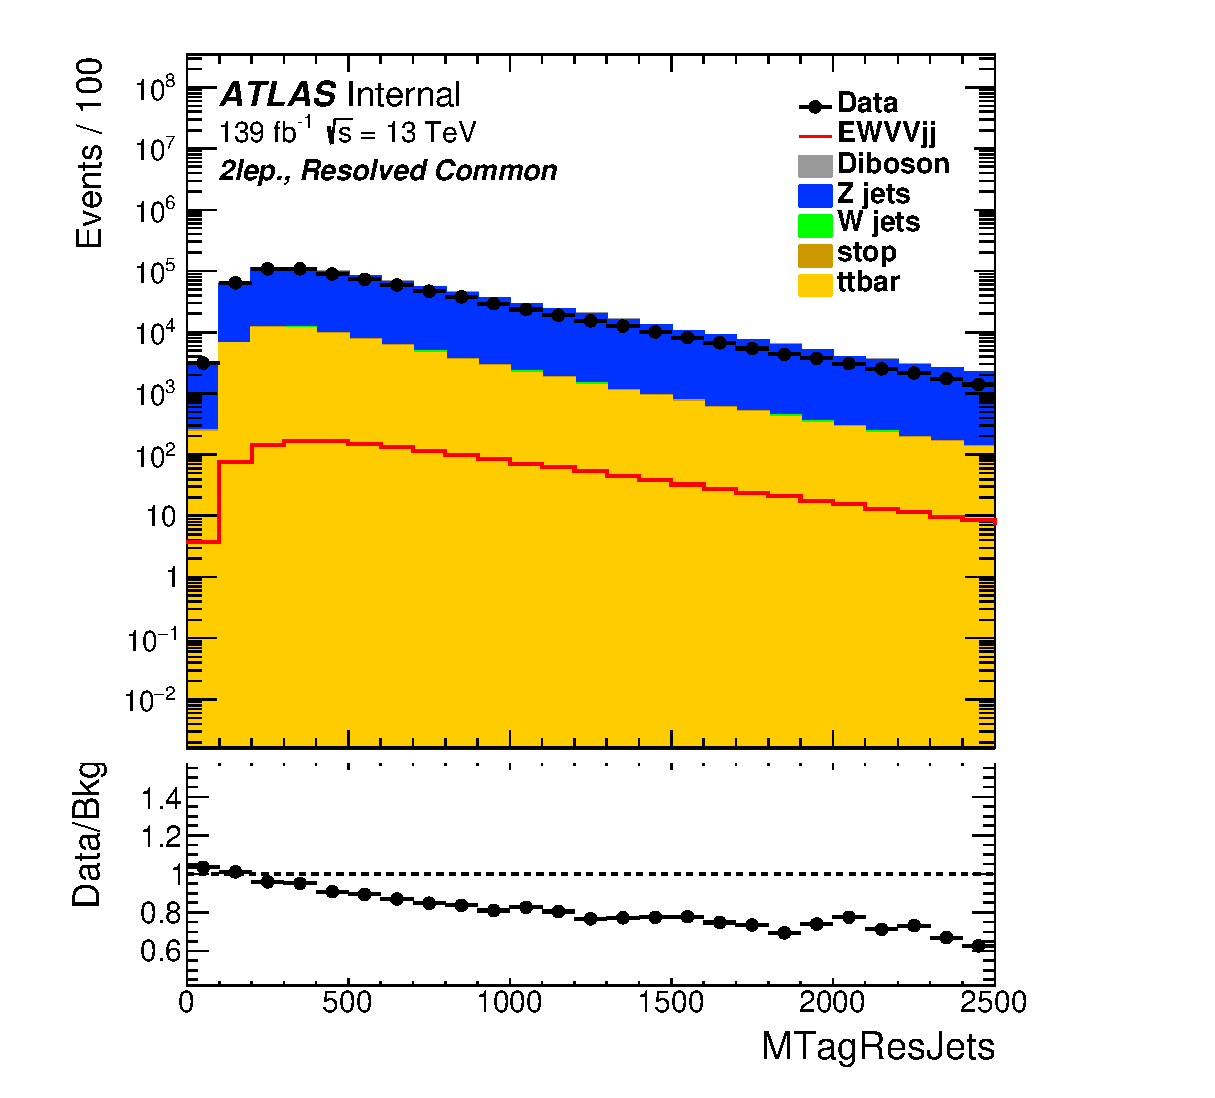
\includegraphics[width=0.4\textwidth]{figures/2lep/dataMC/C_0ptag2pjet_0ptv_ResolvedCommon_MTagResJets_Log} 
    \caption{$m^{tag}_{jj}$ distribution before defining the SRs. The known slope due to the Z+jets modeling issue can be seen. Details are described in Chapter~\ref{}.}
    \label{fig:Mtagjj}
\end{figure}

The $m^{tag}_{jj}$ reweighting, which is described in Chapter~\ref{}, is applied before defining the SRs and CRs to correct the Z+jet modeling.

\section{Hadronically decaying boson, Signal Region (SR) definitions}
Signal regions (SR) are defined to enhance the signal purity, and for background  components the control region (CR). They are defined by requiring the signal jet selections. Defining order starts from merged categories, then move to the resolved category. Each events are categorized into the regions in following order in Figure~\ref{fig:order}. The event selection is performed subsequently, which means only the events failed the previous selection goes to the next selection, therefore there is no events overlapped.
These five regions are simultaneously fitted in the final fitting.

\begin{figure}[H]
    \centering
    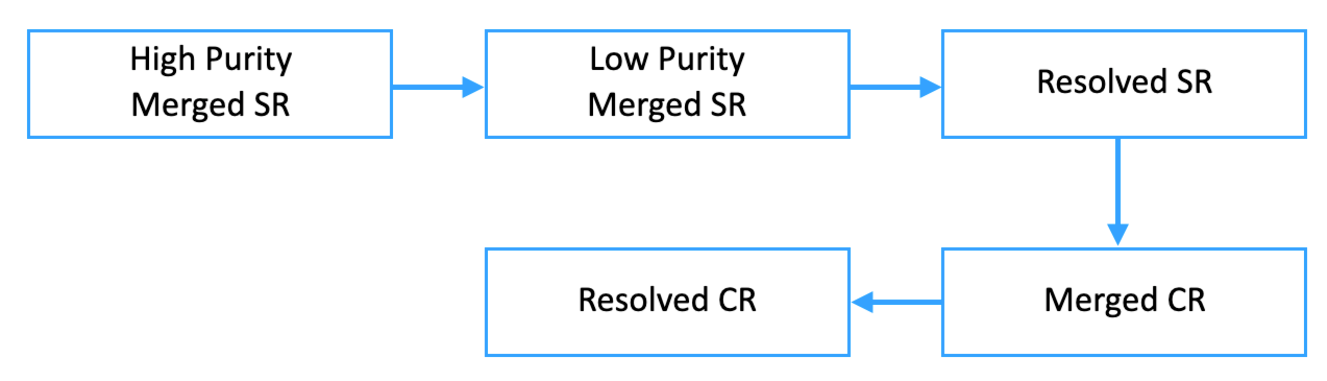
\includegraphics[width=0.8\textwidth]{figures/order}
    \caption{The order of defining the SR and the CR. The merged SR are defined at first, and the events failed the merged SR selections goes to the selection of the resolved SR, therefore there are no overlapped events within several SR and CRs.}
    \label{fig:order}
\end{figure}

\subsection{Merged category}
%merged selection
The hadronic decaying $W/Z$ bosons with $p_{T}(W / Z \rightarrow q q) \geq ~200 \mathrm{GeV}$, can be reconstructed with jets as large-R jets. This merged region requires at least one large-R jet outside of the tagging jets of $|\Delta R|<1.4$. 
The boson-tagger is required to find the reconstructed $W/Z$ bosons and the SRs and CRs are defined. The events passed the boson-tagger working point (WP) at 50$\%$ is categorized to be in the High Purity (HP) Merged SR. The events failed the 50$\%$ WP and passed 80$\%$ goes to the Low Purity (LP) Merged SR. 
The Merged region definition is shown in the Figure~\ref{fig:MergedRegion}.
\begin{figure}[H]
    \centering
    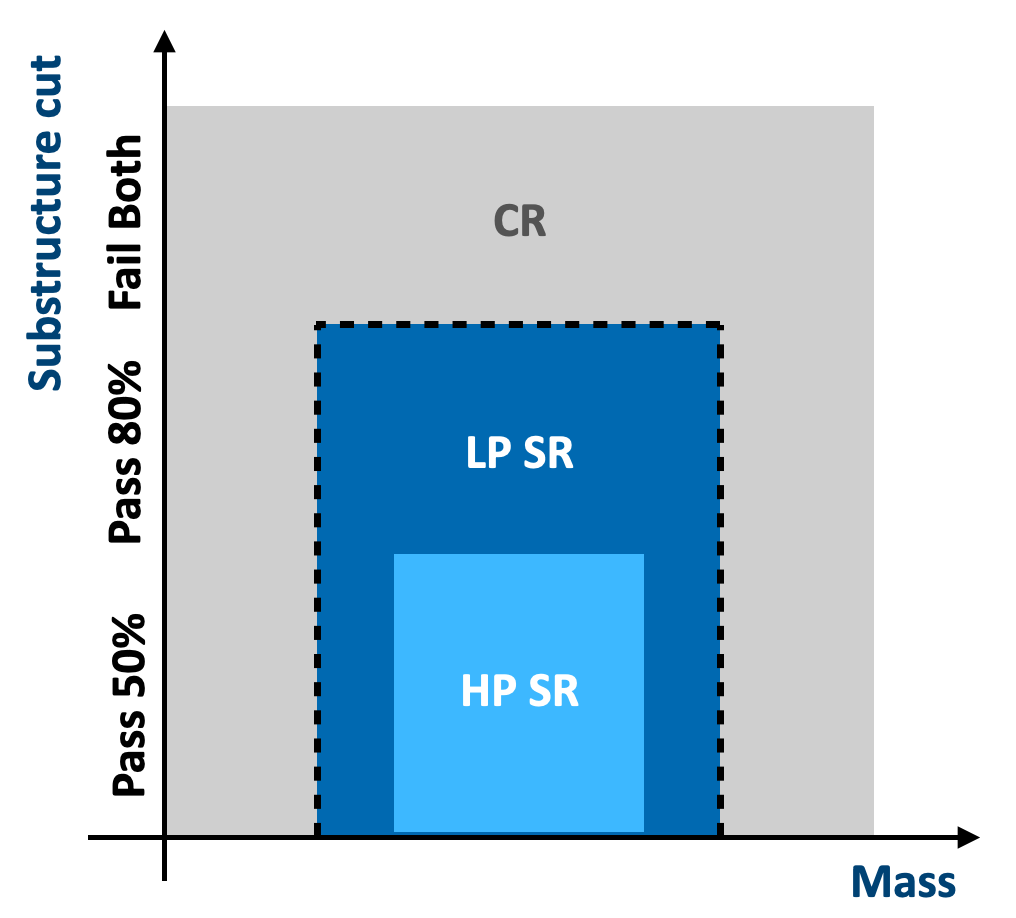
\includegraphics[width=0.6\textwidth]{figures/MergedRegion}
    \caption{The selection of the merged SR and CR are shown. The CR definition is what was changed from the previous round of the analysis, in order to fulfill the requirement to derive the scale factors.}
    \label{fig:MergedRegion}
\end{figure}
The data and MC distribution of the mass of the large-R jet before and after applying the boson tagger is shown in Figure~\ref{fig:2lepfatJet}.
\begin{figure}[H]
    \centering
    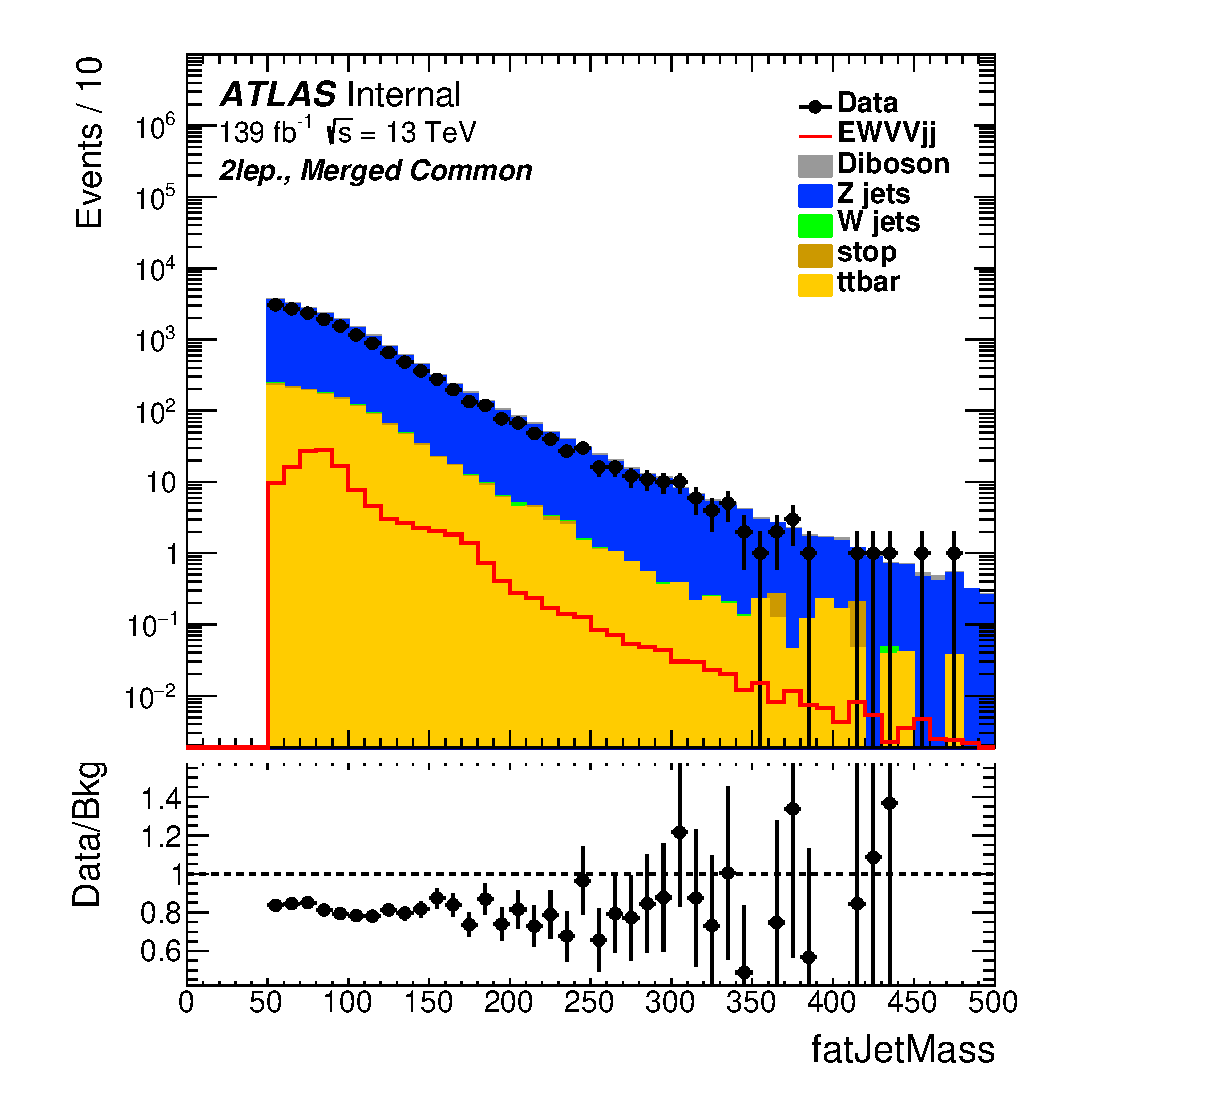
\includegraphics[width=0.4\textwidth]{figures/2lep/dataMC/C_0ptag1pfat0pjet_0ptv_MergedCommon_fatJetMass_Log} \\
    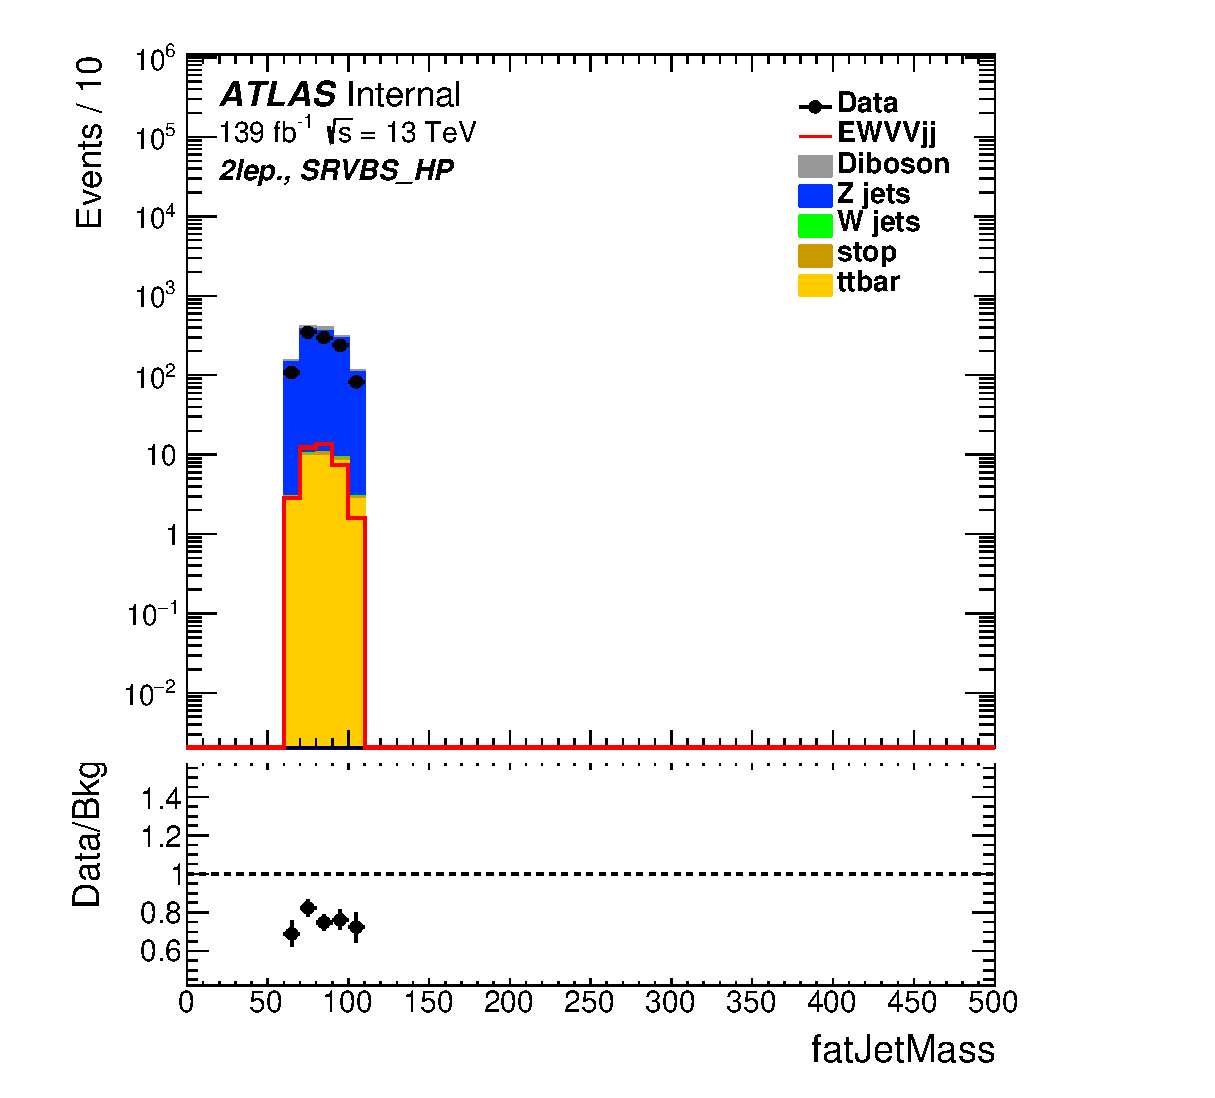
\includegraphics[width=0.4\textwidth]{figures/2lep/dataMC/C_0ptag1pfat0pjet_0ptv_SRVBS_HP_fatJetMass_Log} 
    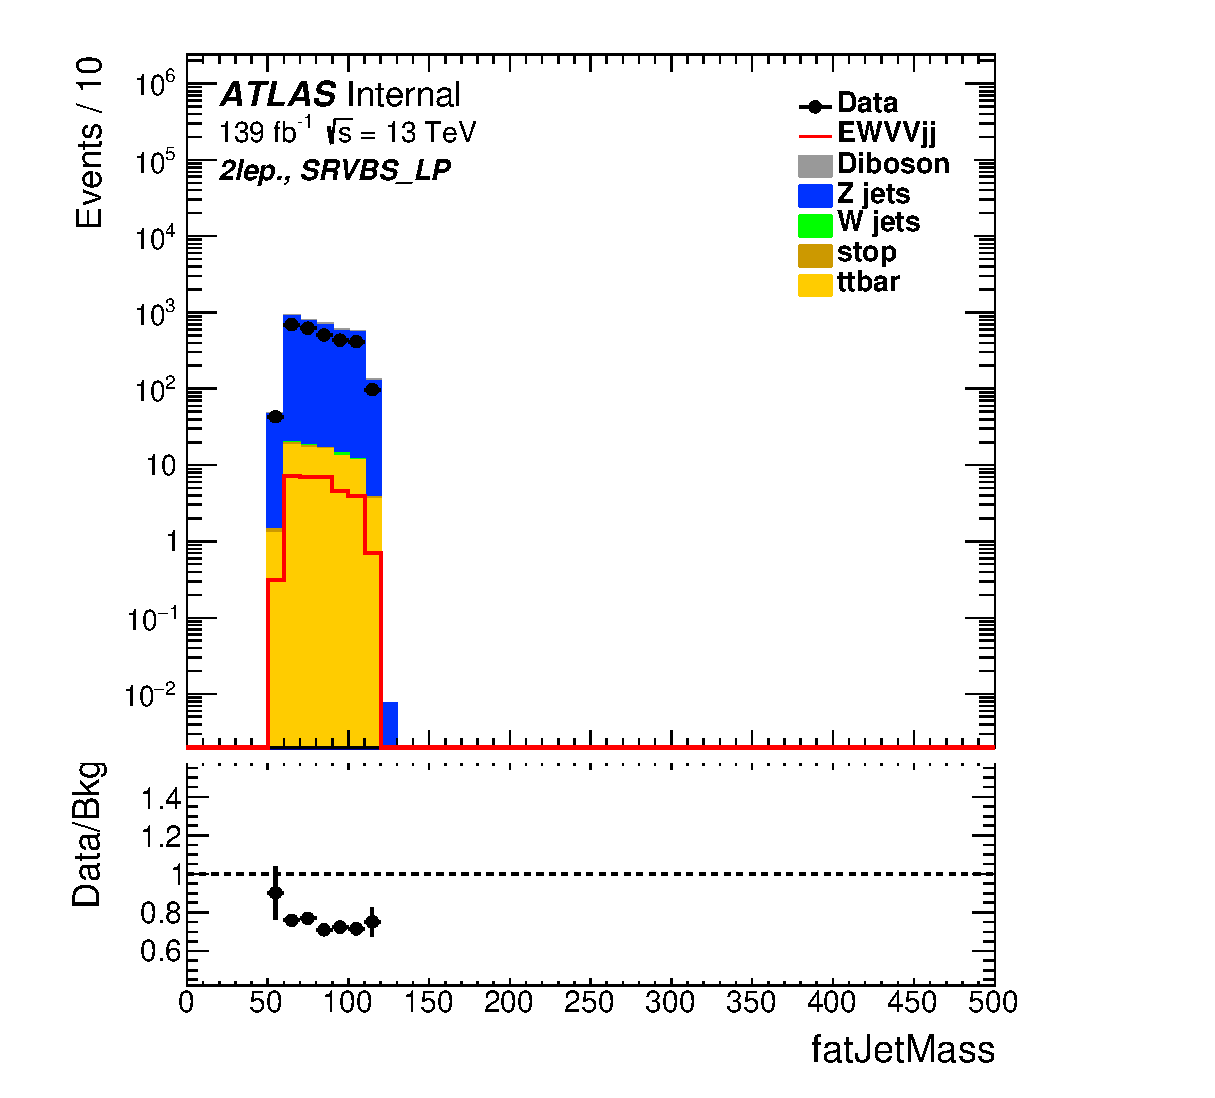
\includegraphics[width=0.4\textwidth]{figures/2lep/dataMC/C_0ptag1pfat0pjet_0ptv_SRVBS_LP_fatJetMass_Log}
    \caption{mass of the large-R jet distribution before and after applying the boson tagger. The boson mass peak can be seen. The second peak shown in the first distribution before applying tagger comes from the top contribution, for example from the process including the Wtb vertex.}
    \label{fig:2lepfatJet}
\end{figure}

The 50~\% working point (WP) $W/Z$-tagging scale factor is applied for the HP SR, and a custom scale factor is defined for the LP SR:
\begin{equation}
S F_{L P}=\frac{\epsilon_{loose} S F_{eff, loose}-\epsilon_{tight} S F_{eff, tight}}{\epsilon_{loose}-\epsilon_{tight}}
\end{equation}
where "loose" refers to the 80\% WP and "tight" refers to the 50\% WP.

The boson-tagger is optimized to maximize the sensitivity to the longitudinally-polarized $W/Z$ bosons. 
The previous study showed that the HPSR is not so sensitive to the fully-transversed aQGC signals, which makes us to keep the LPSR for the aQGC searches. 

\subsection{Resolved category}
For the bosons with the lower $p_T$ ranges, the boson decays into the two well-separated jets. This is cotegorized as resolved region, with having two signal jets. The two leading-$p_T$ small-R jets are selected from the rest of the jets after tagging jets selection. The leading signal jet is required to be $p_T$ > 40~GeV. 
The events are categorized to the resolved SR when pass the mass window of 64 < $m_{jj}$ < 106~GeV. Figure~\ref{fig:MVHadResSR} shows that the reconstructed boson peak before and after requiring the mass window.
\begin{figure}[H]
    \centering
    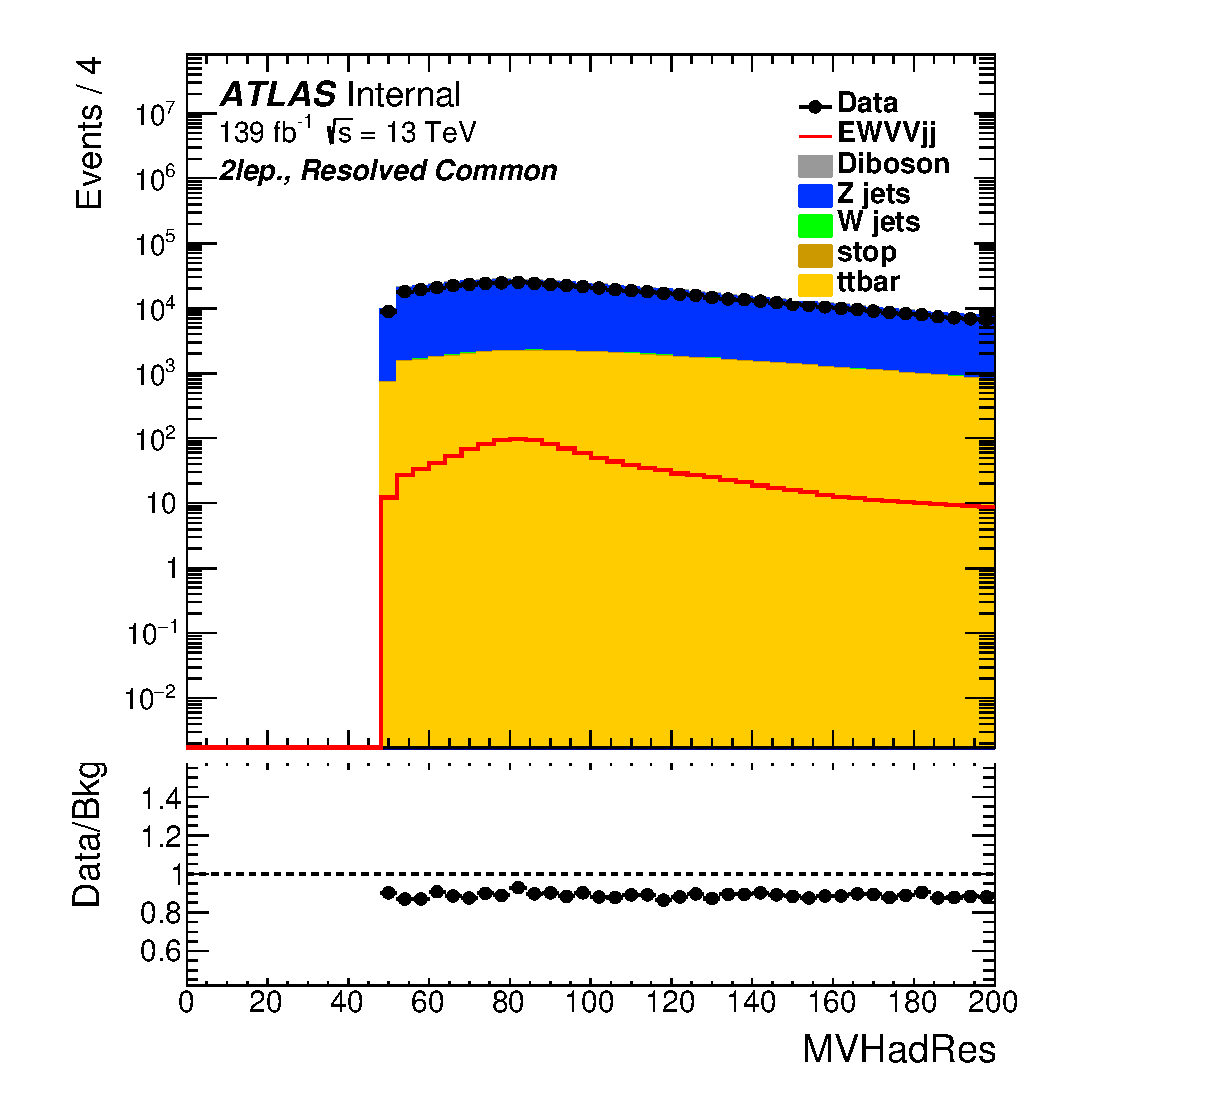
\includegraphics[width=0.4\textwidth]{figures/2lep/dataMC/C_0ptag2pjet_0ptv_ResolvedCommon_MVHadRes_Log}
    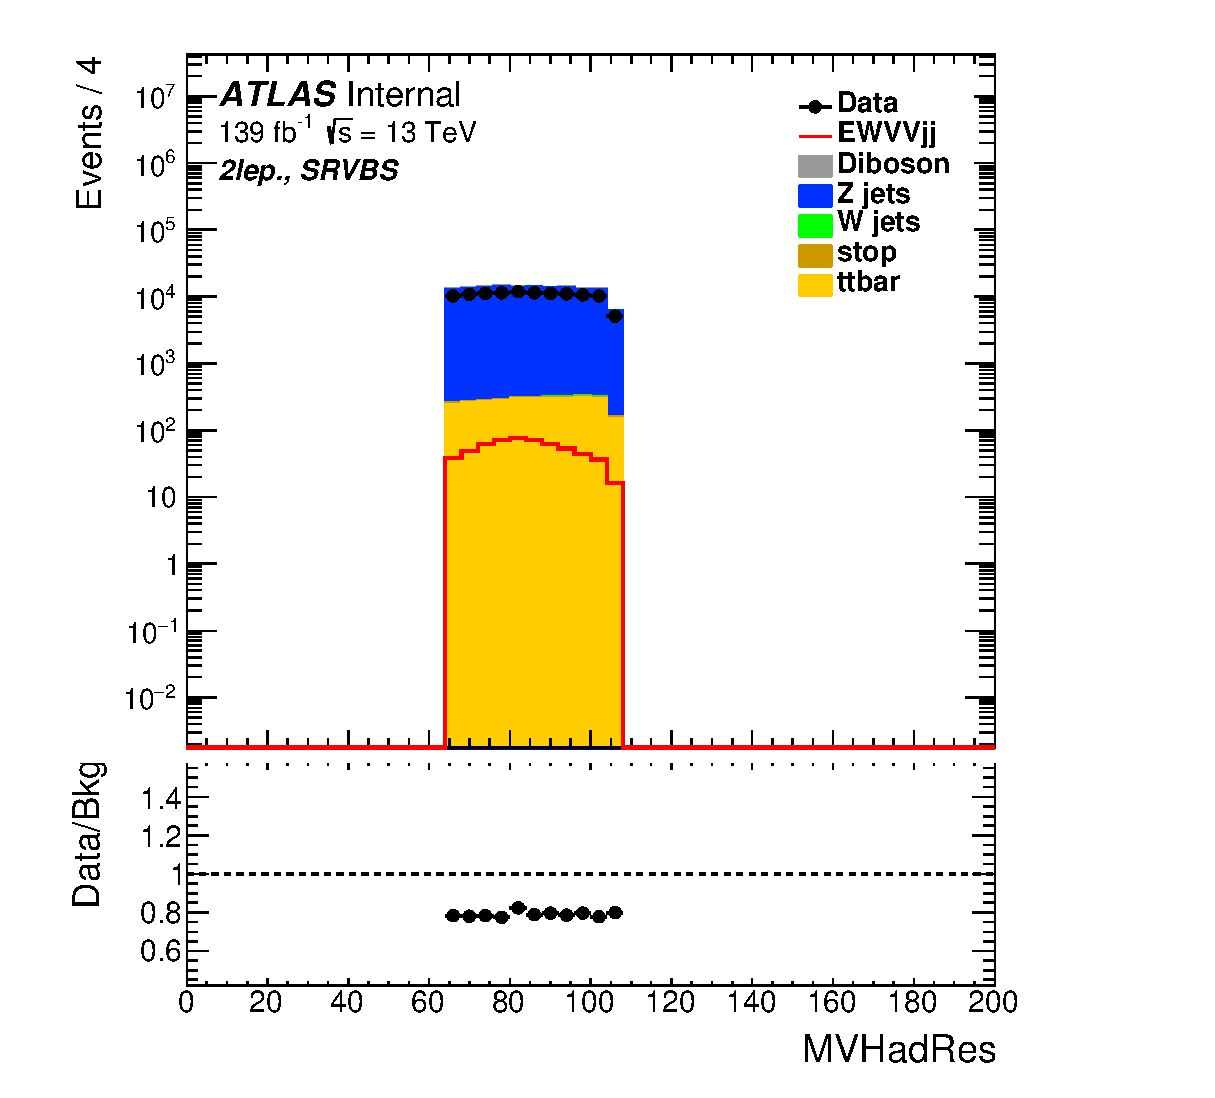
\includegraphics[width=0.4\textwidth]{figures/2lep/dataMC/C_0ptag2pjet_0ptv_SRVBS_MVHadRes_Log}
    \caption{Invariant mass of the two signal jets before and after requiring the mass window. 
    %Before the mass window cut, the $m^{tag}_{jj}$ reweighting is not applied while after mass window cut it is applied, which leads to the difference of the normalization between two plots.
    }
    \label{fig:MVHadResSR}
\end{figure}

After categorization, the invariant mass of the two tagging jets ($\mathrm{m}_{\mathrm{jj}}^{\text {tag}}$) is required to be greater than $400~\mathrm{GeV}$ to enhance the VBS-like topology, both for merged and resolved categories.

\subsection{EW top production veto}
The contribution of the EW top production is found to be still significant after applying the b-veto for the tagging jets, which is about 30~\% of the EW VVjj signal in the resolved category after all SR selections so far.
The additional cut is applied to suppress the top contributions for example tZb diagram from the diagram with the Figure~\ref{fig:feynmantZb} included in the EW VVjj signal sample. The top contribution is not the VBS diagrams, while we cannot separate this diagram from VBS ones in the gauge invariant way. Therefore a cut to the reconstructed top mass,$m_{jjj}$ > 200~GeV is decided to be applied. The $m_{jjj}$ is derived with the two signal jets and the third jet which forms the three-jet mass, the closest to the Top mass (172.76~GeV). The $m_{jjj}$ with events with each truth particles is shown, and the modeling plot is also shown in Figure~\ref{fig:2leptopMass}. 
\begin{figure}[H]
    \begin{center}
      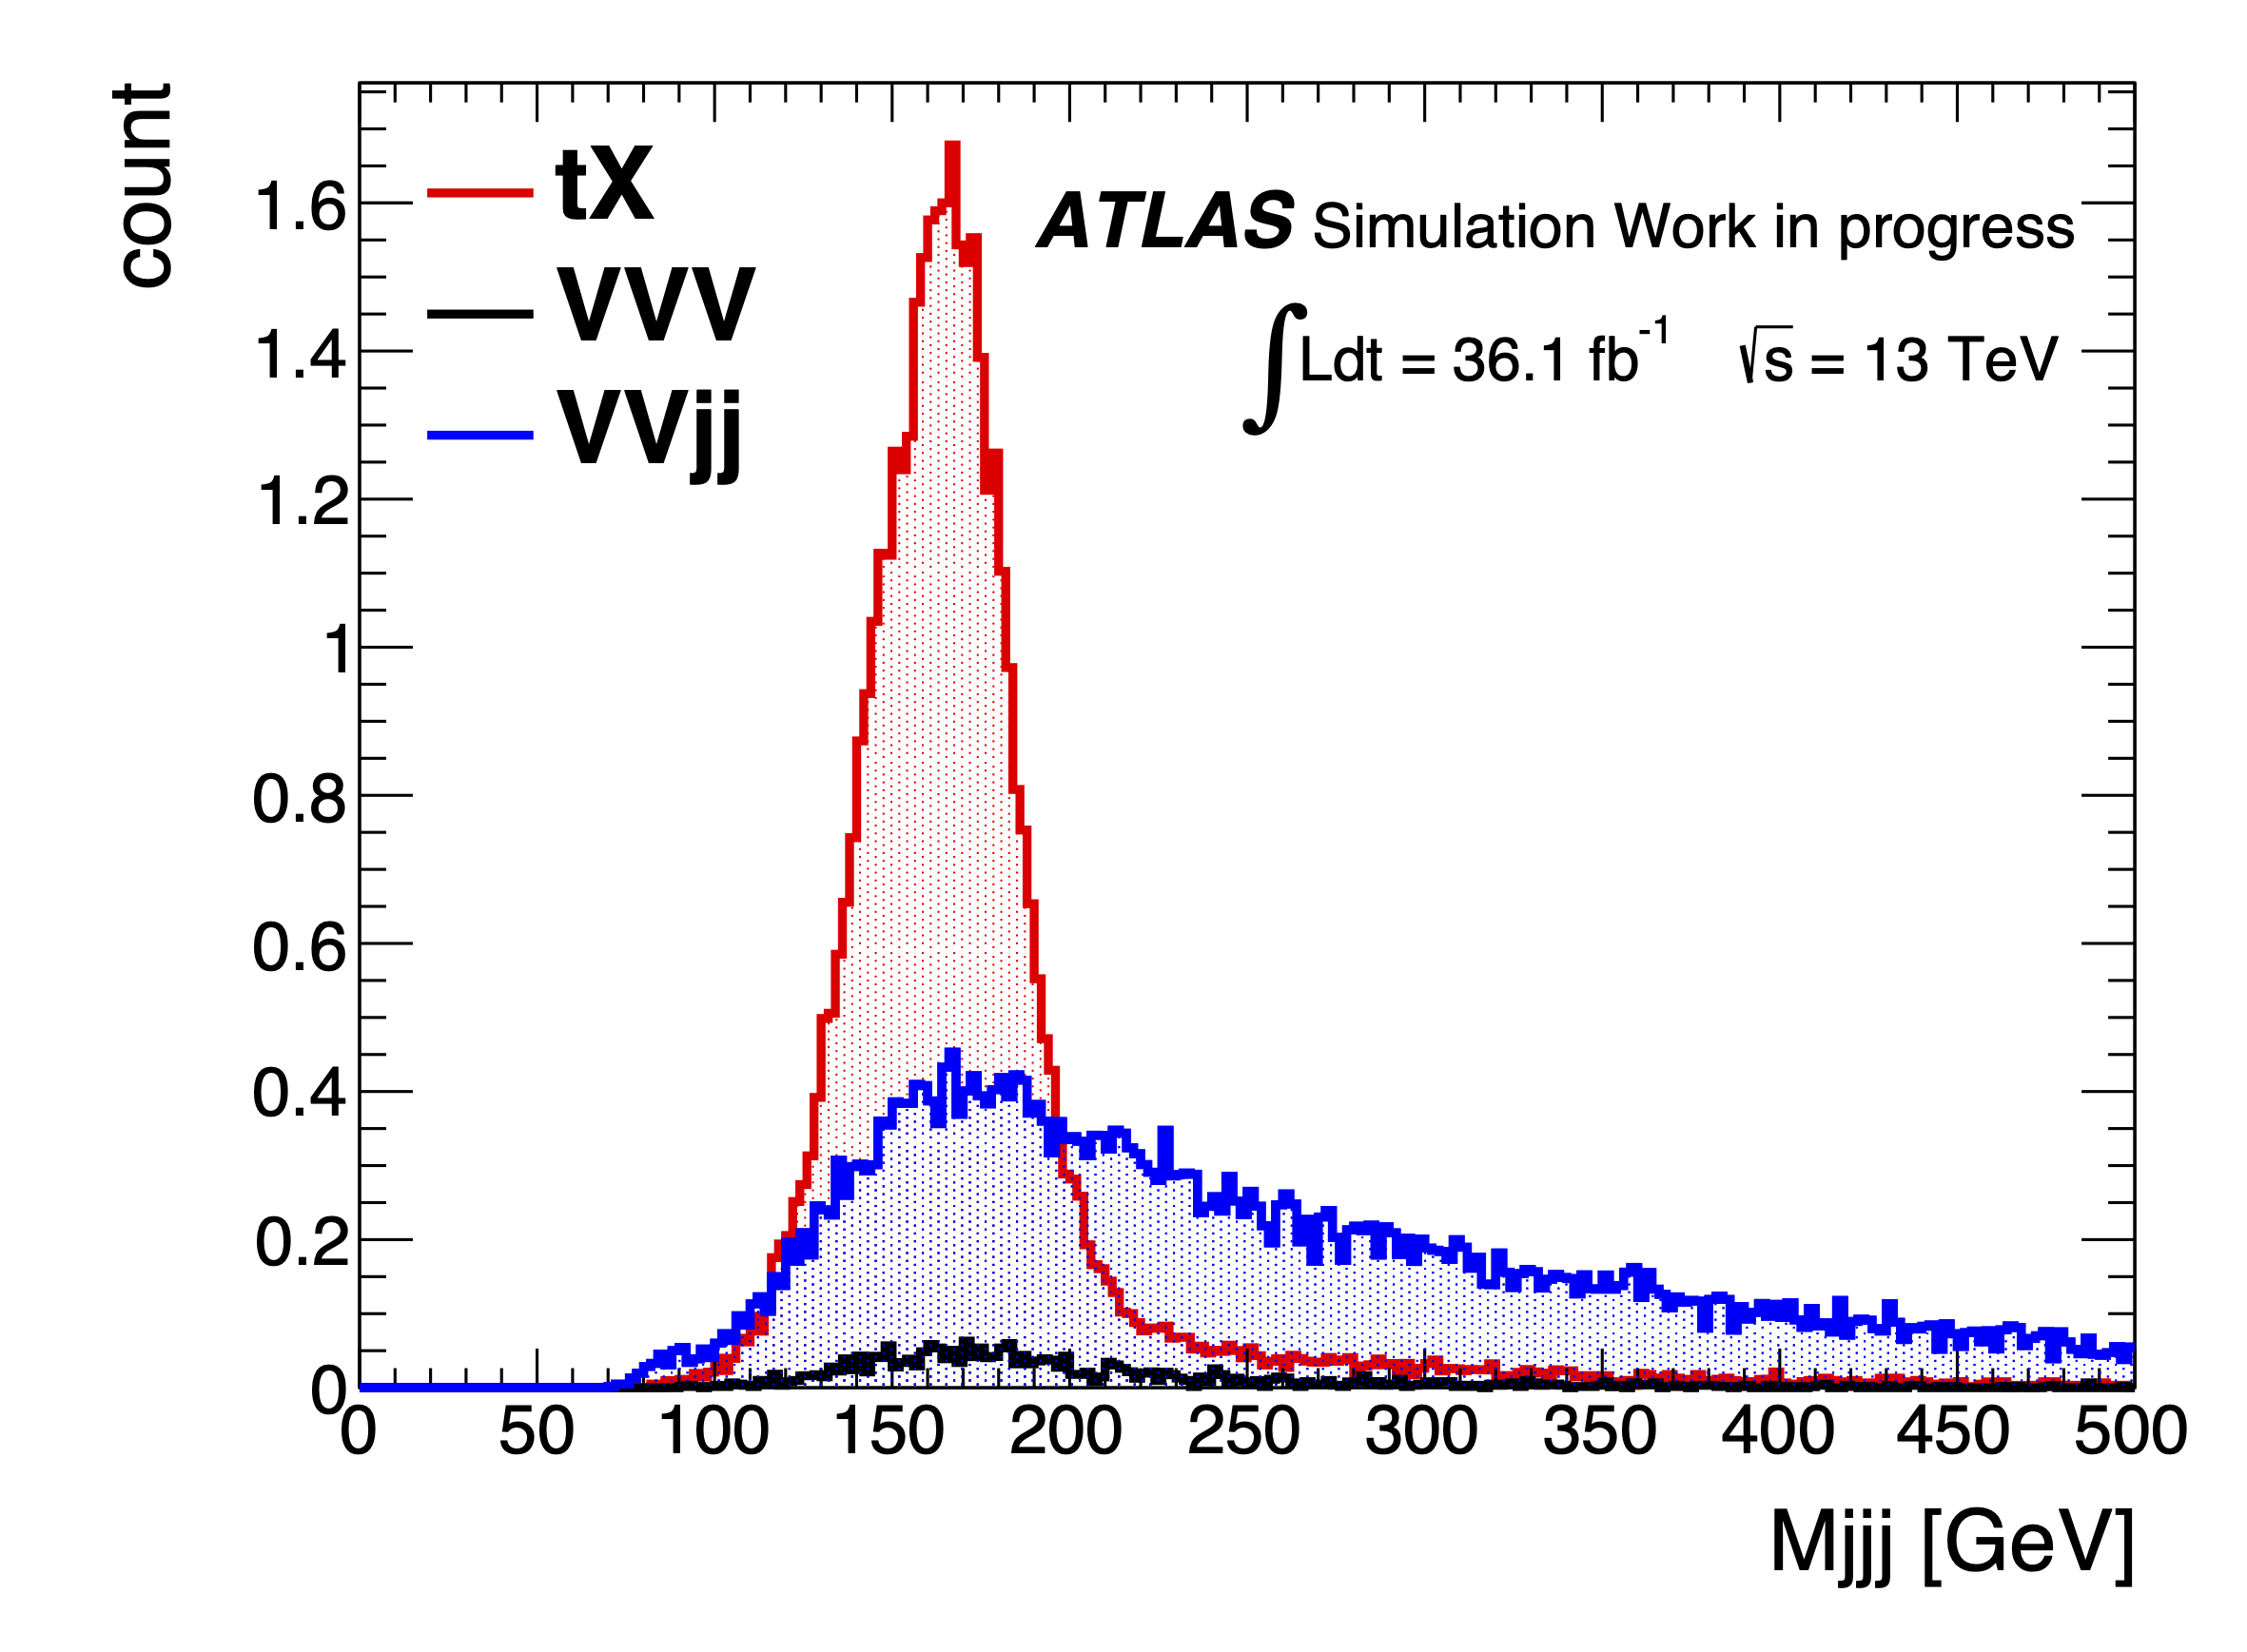
\includegraphics[width=0.45\textwidth]{figures/2lep/topMass/WZjjtopMasspeak}
      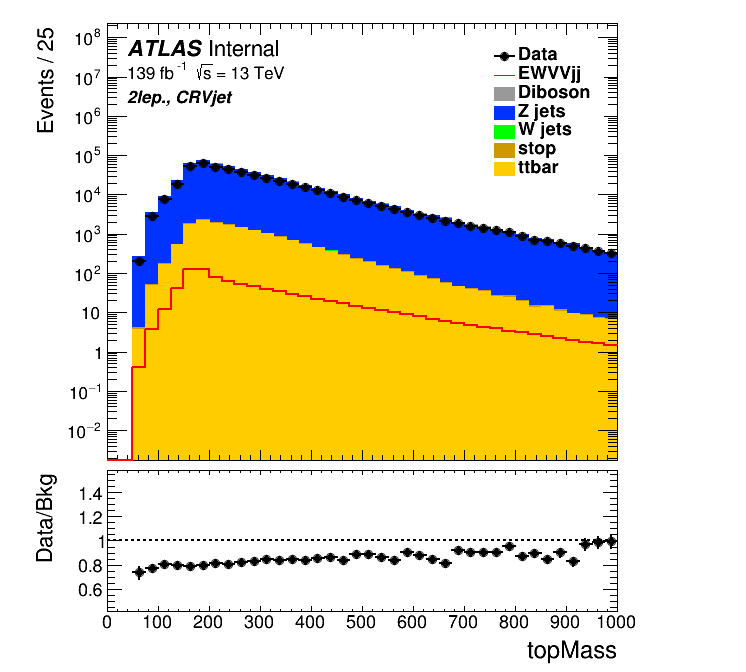
\includegraphics[width=0.45\textwidth]{figures/2lep/dataMC/C_0ptag2pjet_0ptv_CRVjet_topMass_Log}
        \caption{ Mass of 3 jets in the 2-lepton channel CRVjet.}
        \label{fig:2leptopMass}
    \end{center}
\end{figure}
This top-mass cut can reduce the top contributions, as shown in Table~\ref{fig:TruthTop2LepPurity} in resolved category, therefore the resolved SR is defined with this additional cut to get more VBS-like phase space. In merged category top-mass cut does little thing to enhance the VBS signals since top contribution is already small without the top mass cut, hence this cut is not added to the merged SR definition.
\begin{figure}[H]
    \centering
    \resizebox{0.95\textwidth}{!}{
    \begin{tabular}{|c||c|c|c|c|}
         \hline
                        & SRVBS (resolved) & VBS enhanced (resolved) & SRVBS (merged) & VBS enhanced (merged) \\ \hline
        Truth Top       & 0.48             & 0.14                    & 0.14           & 0.10                  \\ \hline
        Truth VVV       & 0.03             & 0.03                    & 0.08           & 0.08                  \\ \hline
        Truth VBS       & 0.49             & 0.83                    & 0.78           & 0.82                  \\ \hline
    \end{tabular}
        }
        \caption{Fraction of event yields for 2lepton channel. The truth information is used to know if the event includes each contributions. Only EWWZjj events are checked here since there are no Top contributions in EWZZjj events.}
        \label{fig:TruthTop2LepPurity}
\end{figure}

\section{Control Region (CR) definitions}
$V+jets$ CR is defined to constrain the normalization of the backgrounds. For 2-lepton channel, V means Z, which is the main background.
%V+jets CR
For the merged CRs, the single V+jets CRs are defined for the events failing the 80$\%$ WP of the boson tagger. Resolved CRs are defined with using the mass sideband. It is defined with the same event selection as the resolved SR but outside the mass window, which is $50<m_{i i}<64 ~\mathrm{GeV}$, or $m_{i i}>106 ~\mathrm{GeV}$.
The data/MC distribution with respect to the hadronically decaying boson mass for resolved CRs is shown in Figure~\ref{fig:CRVjet}.
\begin{figure}[H]
    \centering
    %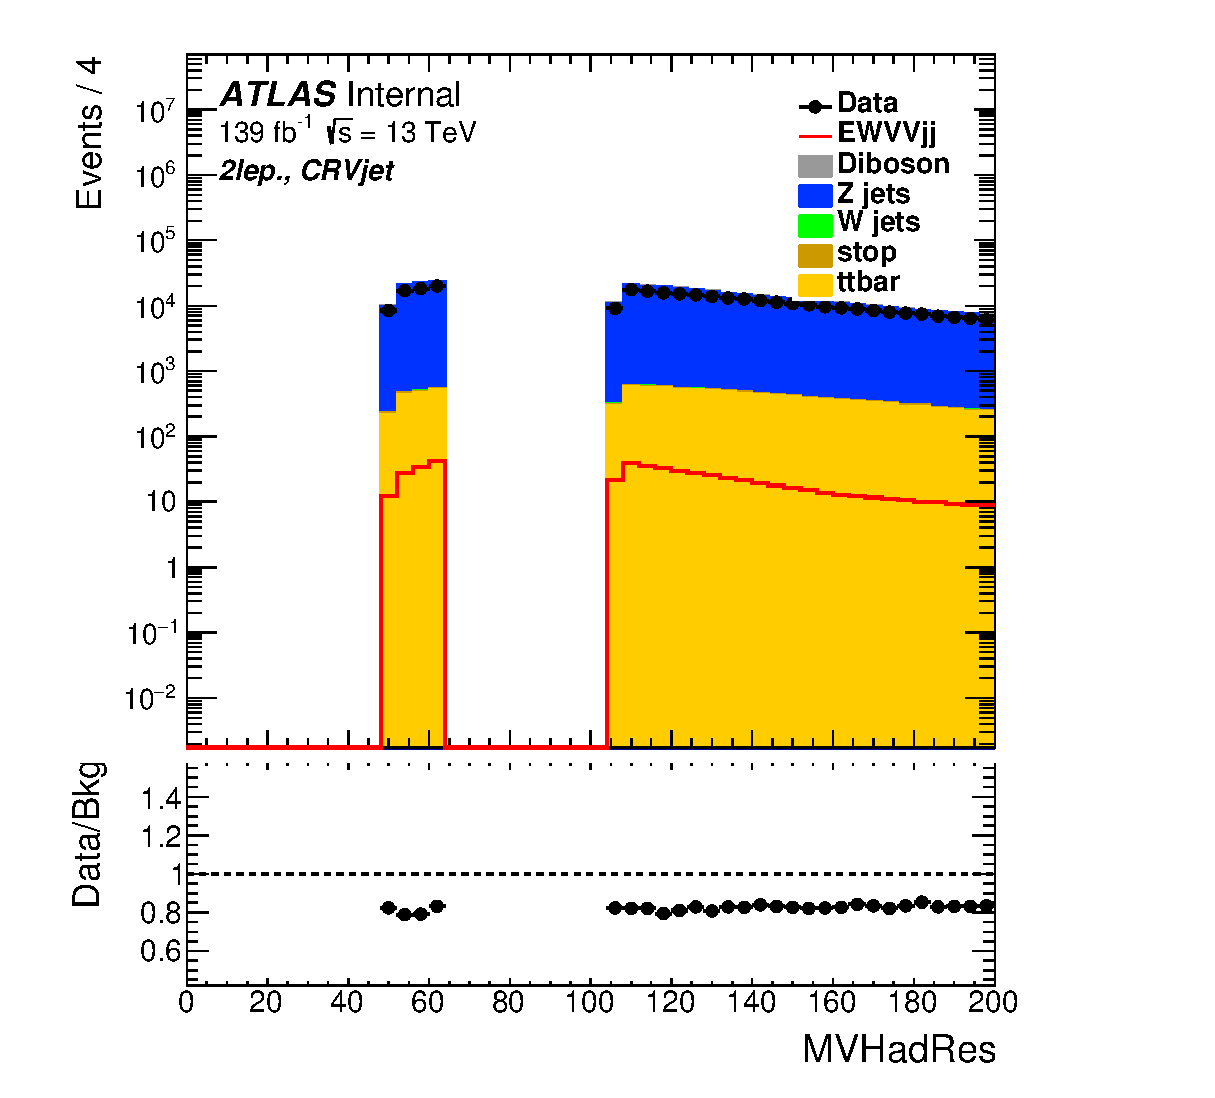
\includegraphics[width=0.4\textwidth]{figures/2lep/dataMC/C_0ptag2pjet_0ptv_CRVjet_MVHadRes_Log}
    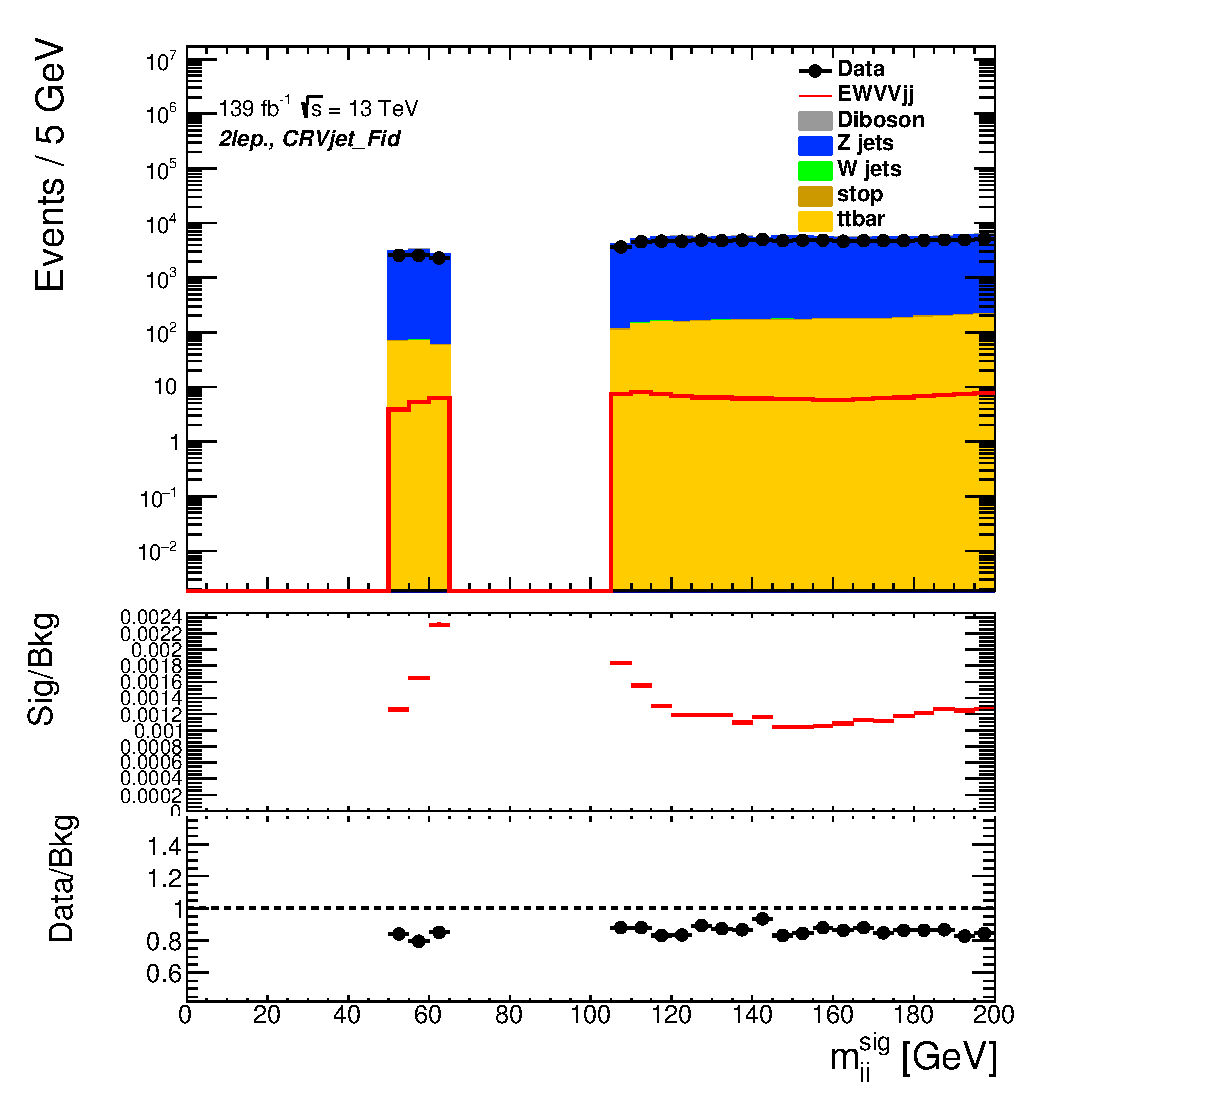
\includegraphics[width=0.4\textwidth]{figures/2lep/dataMC/C_0ptag2pjet_0ptv_CRVjet_Fid_MVHadRes_Log}
    \caption{Mass of reconstructed boson in the resolved CR}
    \label{fig:CRVjet}
\end{figure}

In the merged CR, the inefficiency scale factors $SF_{ineff,loose}$ calaculated for the 80\% working point tagger are applied:
\begin{equation}
S F_{i n e f f}=\frac{1-\epsilon \times S F_{e f f}}{1-\epsilon}
\end{equation}
where $\epsilon$ is the efficiency estimated in ttbat events for signal and $\gamma$+jet and multi-jet events for background.
%%%%%%%%%%%%
%\noindent \textbf{0-lepton}\\
%The $Z \rightarrow \nu\nu$ identification requires no Loose lepton and high missing energy (E$_T^{miss}$ > 200~GeV) in the final state. There are significant QCD multijet background in 0-lepton channel, therefore some cuts suppressing the multijets are applied: \\
%\\
%- $p_{\mathrm{T}}^{\mathrm{miss}}>50 \mathrm{GeV}$ \\
%- $\Delta \phi\left(E_{\mathrm{T}}^{\mathrm{miss}}, p_{\mathrm{T}}^{\mathrm{miss}}\right)<\pi / 2$ \\
%- $\min \left(\Delta \phi\left(E_{\mathrm{T}}^{\mathrm{miss}}, j\right)\right)>\pi / 6$ \\
%- $\Delta \phi\left(E_{\mathrm{T}}^{\mathrm{miss}}, \overrightarrow{\mathbf{V}}_{\mathrm{had}}\right)>\pi / 9$ \\ \\
%where $p_{\mathrm{T}}^{\mathrm{miss}}$ is the track-based missing momentum, and $\min \left(\Delta \phi\left(E_{\mathrm{T}}^{\mathrm{miss}}, j\right)\right)$ is the minimum azimuthal difference betwween $E_{\mathrm{T}}^{\mathrm{miss}}$ and small-R jets. \\

%\noindent\textbf{1-lepton} \\
%To select the events with $W \rightarrow l\nu$ candidate, exactly one Tight lepton is required.
%In order to suppress the multi-jet background, following cuts are applied for all regions: \\ \\
%- $E_{\mathrm{T}}^{\text {miss }}>80 \mathrm{GeV}$ \\ 
%- $p_{\mathrm{T}, \ell}>28 \mathrm{GeV}$ \\
%- $m_{J}>50 \mathrm{GeV}$ (merged only) \\ \\

%\noindent\textbf{2-lepton} \\
%The $Z \rightarrow ll$ candidates are selected by requiring two isolated same-flavour Loose leptons. Both leptons required to be $p_T$ > 27~GeV. Opposite charges are required only for muons and not for electrons, since electrons are more sensitive to charge mis-identification due to the conversions of photons from bremsstrahlung, especially at high $E_T$.
%The $m_{ll}$, invariant mass of the dilepton is required to be in the mass window \\ \\
%- $83 < m_{ee}< 99~GeV$ \\ 
%- $\left(85.6-0.0117 p_{\mathrm{T}, \ell \ell}\right)<m_{\mu \mu}<\left(94.0+0.0185 p_{\mathrm{T}, \ell \ell}\right) \mathrm{GeV}$ \\ \\
%The second equation for muons was oprimized from the 2015+16 analysis~\cite{}. 
%The modeling distribution of lepton distribution in the early stage of the selection is shown in Figure~\ref{fig:2lepLeptons}. The mass peak of Z boson can be seen here.

%\begin{figure}[ht]
%    \centering
%    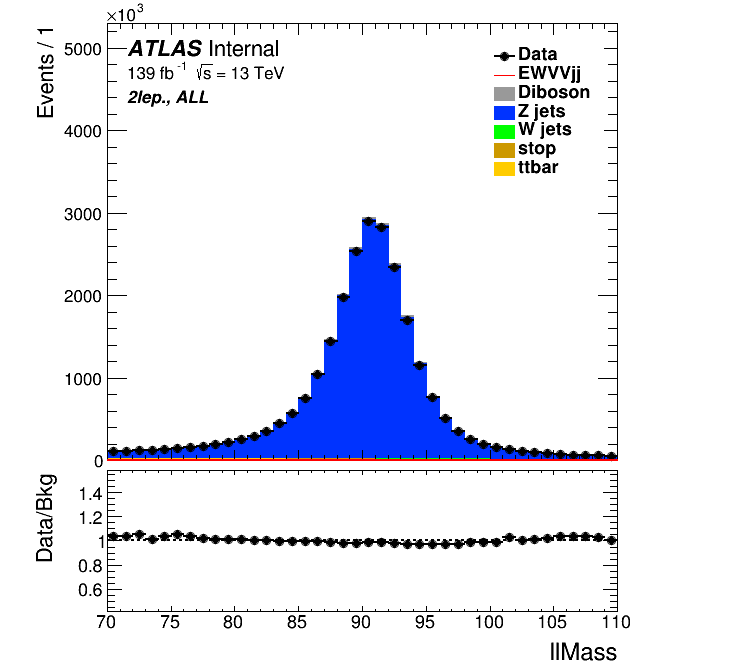
\includegraphics[width=0.5\textwidth]{figures/2lep/dataMC/C_0ptag1pfat0pjet_0ptv_ALL_llMass_Lin}
%    \caption{Lepton distributions in 2-lepton channel. The events before any selections are shown. Z mass peak is shown in $M_{ll}$ distribution.}
%    \label{fig:2lepLeptons}
%\end{figure}

%\section{Signal Regions and Control Regions}
%In all three channels events are required to have a small-R jets pair as a candidate of the forward jets, referred as tagging jets. The another jets pair which is the candidate of the jets hadronically decayed from $W/Z$boson, referred as signal jet is selected as two small-R jets or one large-R jet.
%tagging jet selection
%There needs to be at least four jets, and the tagging jets are first to be selected. Tagging-jets are required to be b-vetoed, which means to be not b-tagged to suppress the contribution of the $Wtb$ vertex in the electroweak VVjj signals. Additionally the fJVT selection is applied to the all small-R jets, with fJVT Loose working point (WP). Tagging jets are selected from the opposite hemispheres, $\eta_{\operatorname{tag} j_{1}} \cdot \eta_{\operatorname{tag} j_{2}}<0$, and to have the highest dijet invariant mass, and each tagging jet is required to be $p_T$ > 30~GeV.

%how to define SR and
%Signal regions (SR) are defined to enhance the signal purity, and for background  components the control region (CR). There are SR and CRs separately in the merged regions and the resolved regions.
%Each events are categorized into the regions in following order in Figure~\ref{fig:order}. These five regions are simultaneously fitted in the final fitting.

%\begin{figure}[ht]
%    \centering
%    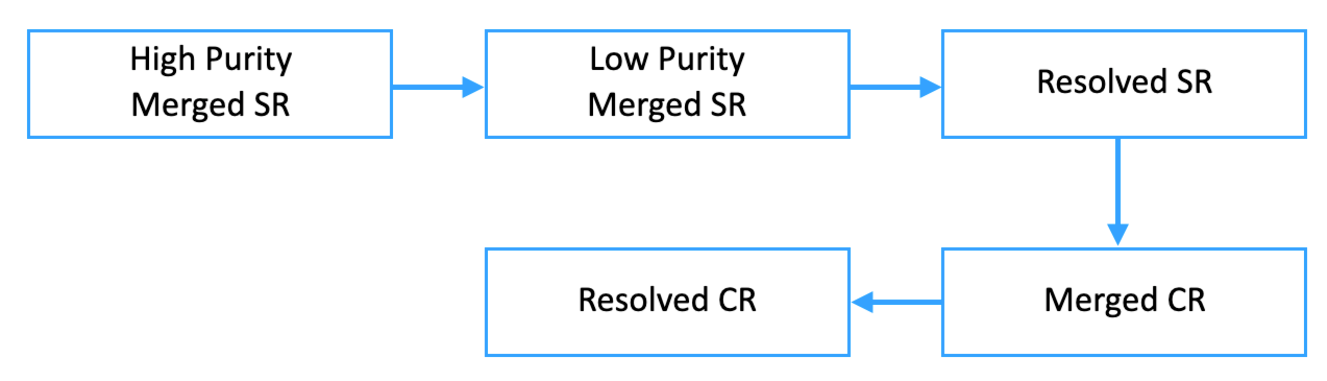
\includegraphics[width=0.8\textwidth]{figures/order}
%    \caption{The order of defining the SR and the CR. The merged SR are defined at first, and the events %failed the merged SR selections goes to the selection of the resolved SR, therefore there are no %overlapped events within several SR and CRs.}
%    \label{fig:order}
%\end{figure}

%merged selection
%The hadronic decaying $W/Z$ bosons with $p_{T}(W / Z \rightarrow q q) \geq 200 \mathrm{GeV}$, can be reconstructed with jets as large-R jets. This merged region required at least one large-R jet outside of the tagging jets of $|\Delta R|<1.4$. 
%The boson-tagger is required to find the reconstructed $W/Z$ bosons and the SRs and CRs are defined. The boson-tagger is based on the three variables; jet mass, $D_2$ and $n_Tracks$. The events passed the boson-tagger working point (WP) at 50$\%$ is categorized to be in the High Purity (HP) Merged SR. The events failed the 50$\%$ WP and passed 80$\%$ goes to the Low Purity (LP) Merged SR. 
%The boson-tagger is optimized to maximize the sensitivity to the longitudinally-polarized $W/Z$ bosons. 
%The previous study showed that the HPSR is not so sensitive to the fully-transversed aQGC signals, which makes us to keep the LPSR for the aQGC searches. 
%put here the reference!
%The Merged region definition is shown in the Figure~\ref{fig:MergedRegion}.
%\begin{figure}[ht]
%    \centering
%    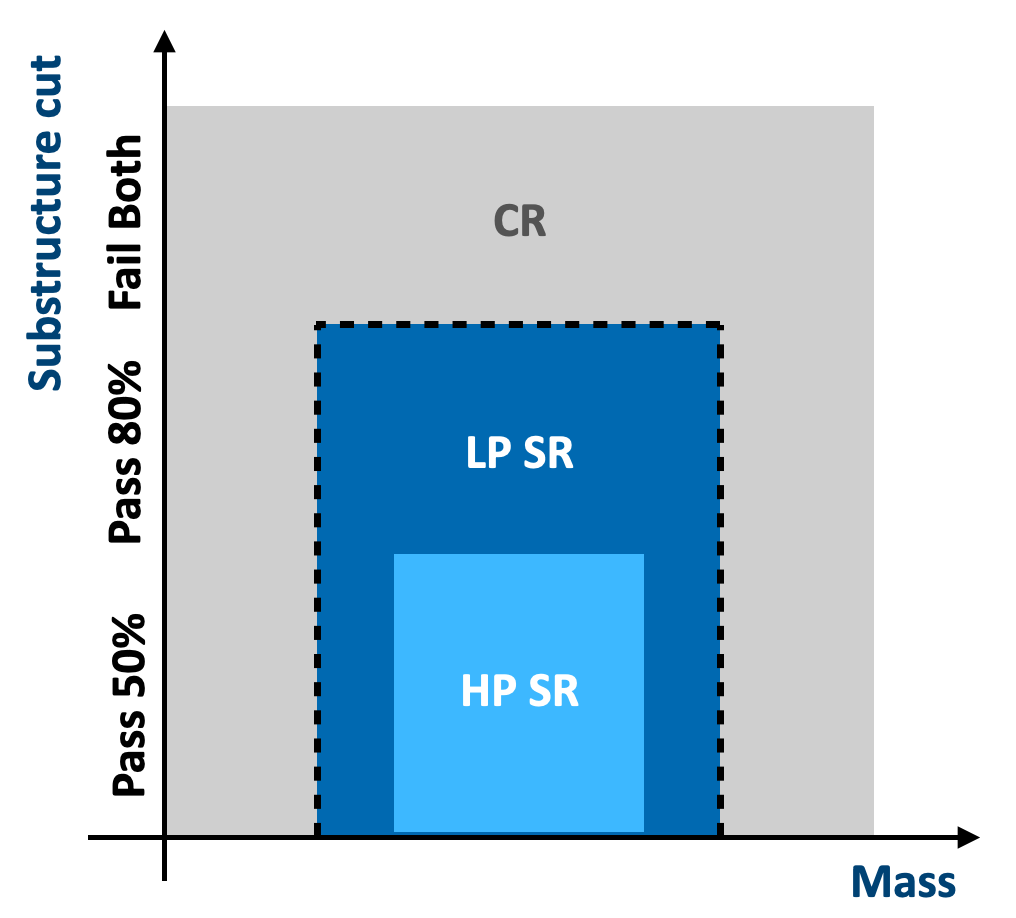
\includegraphics[width=0.6\textwidth]{figures/MergedRegion}
%    \caption{The selection of the merged SR and CR are shown. The CR definition is what was changed from %the previous round of the analysis, in order to fulfill the requirement to derive the scale factors.}
%    \label{fig:MergedRegion}
%\end{figure}


%resolved selection
%For the bosons with the lower $p_T$ ranges, the boson decays into the two well-separated jets. This is cotegorized as resolved region, with having two signal jets. The two small-R jets are selected from the rest of the jets after tagging jets selection. The leading signal jet is required to be $p_T$ > 40~GeV. The events are categorized to the resolved SR when pass the mass window of 64 < $m_{jj}$ 106~GeV. Figure~\ref{fig:MVHadResSR} shows that the reconstructed boson peak.
%This signal-jet selecting strategy is changed from the previous round of the analysis..
%VBS selection and top veto cut
%The event selection is applied to enhance the VBS topology. After categorization the invariant mass of %the two tagging jets ($\mathrm{m}_{\mathrm{jj}}^{\text {tag }}$) is greater than $400 \mathrm{GeV}$.
%The additional cut is applied to suppress the top contributions for example tZb diagram from the diagram with the Figure~\ref{fig:feynmantZb} included in the signal sample. The top contribution is not the VBS diagrams, while we cannot separate this diagram in the gauge invariant way. Therefore we decided to reconstruct the top mass with the two signal jets and the third jet which forms the three-jet mass, $m_{jjj}$, the closest to the Top mass (172.76~GeV). The $m_{jjj}$ with events with each truth particles is shown, and the modeling plot is also shown in Figure~\ref{fig:2leptopMass}. 
%\begin{figure}[ht]
%    \begin{center}
%      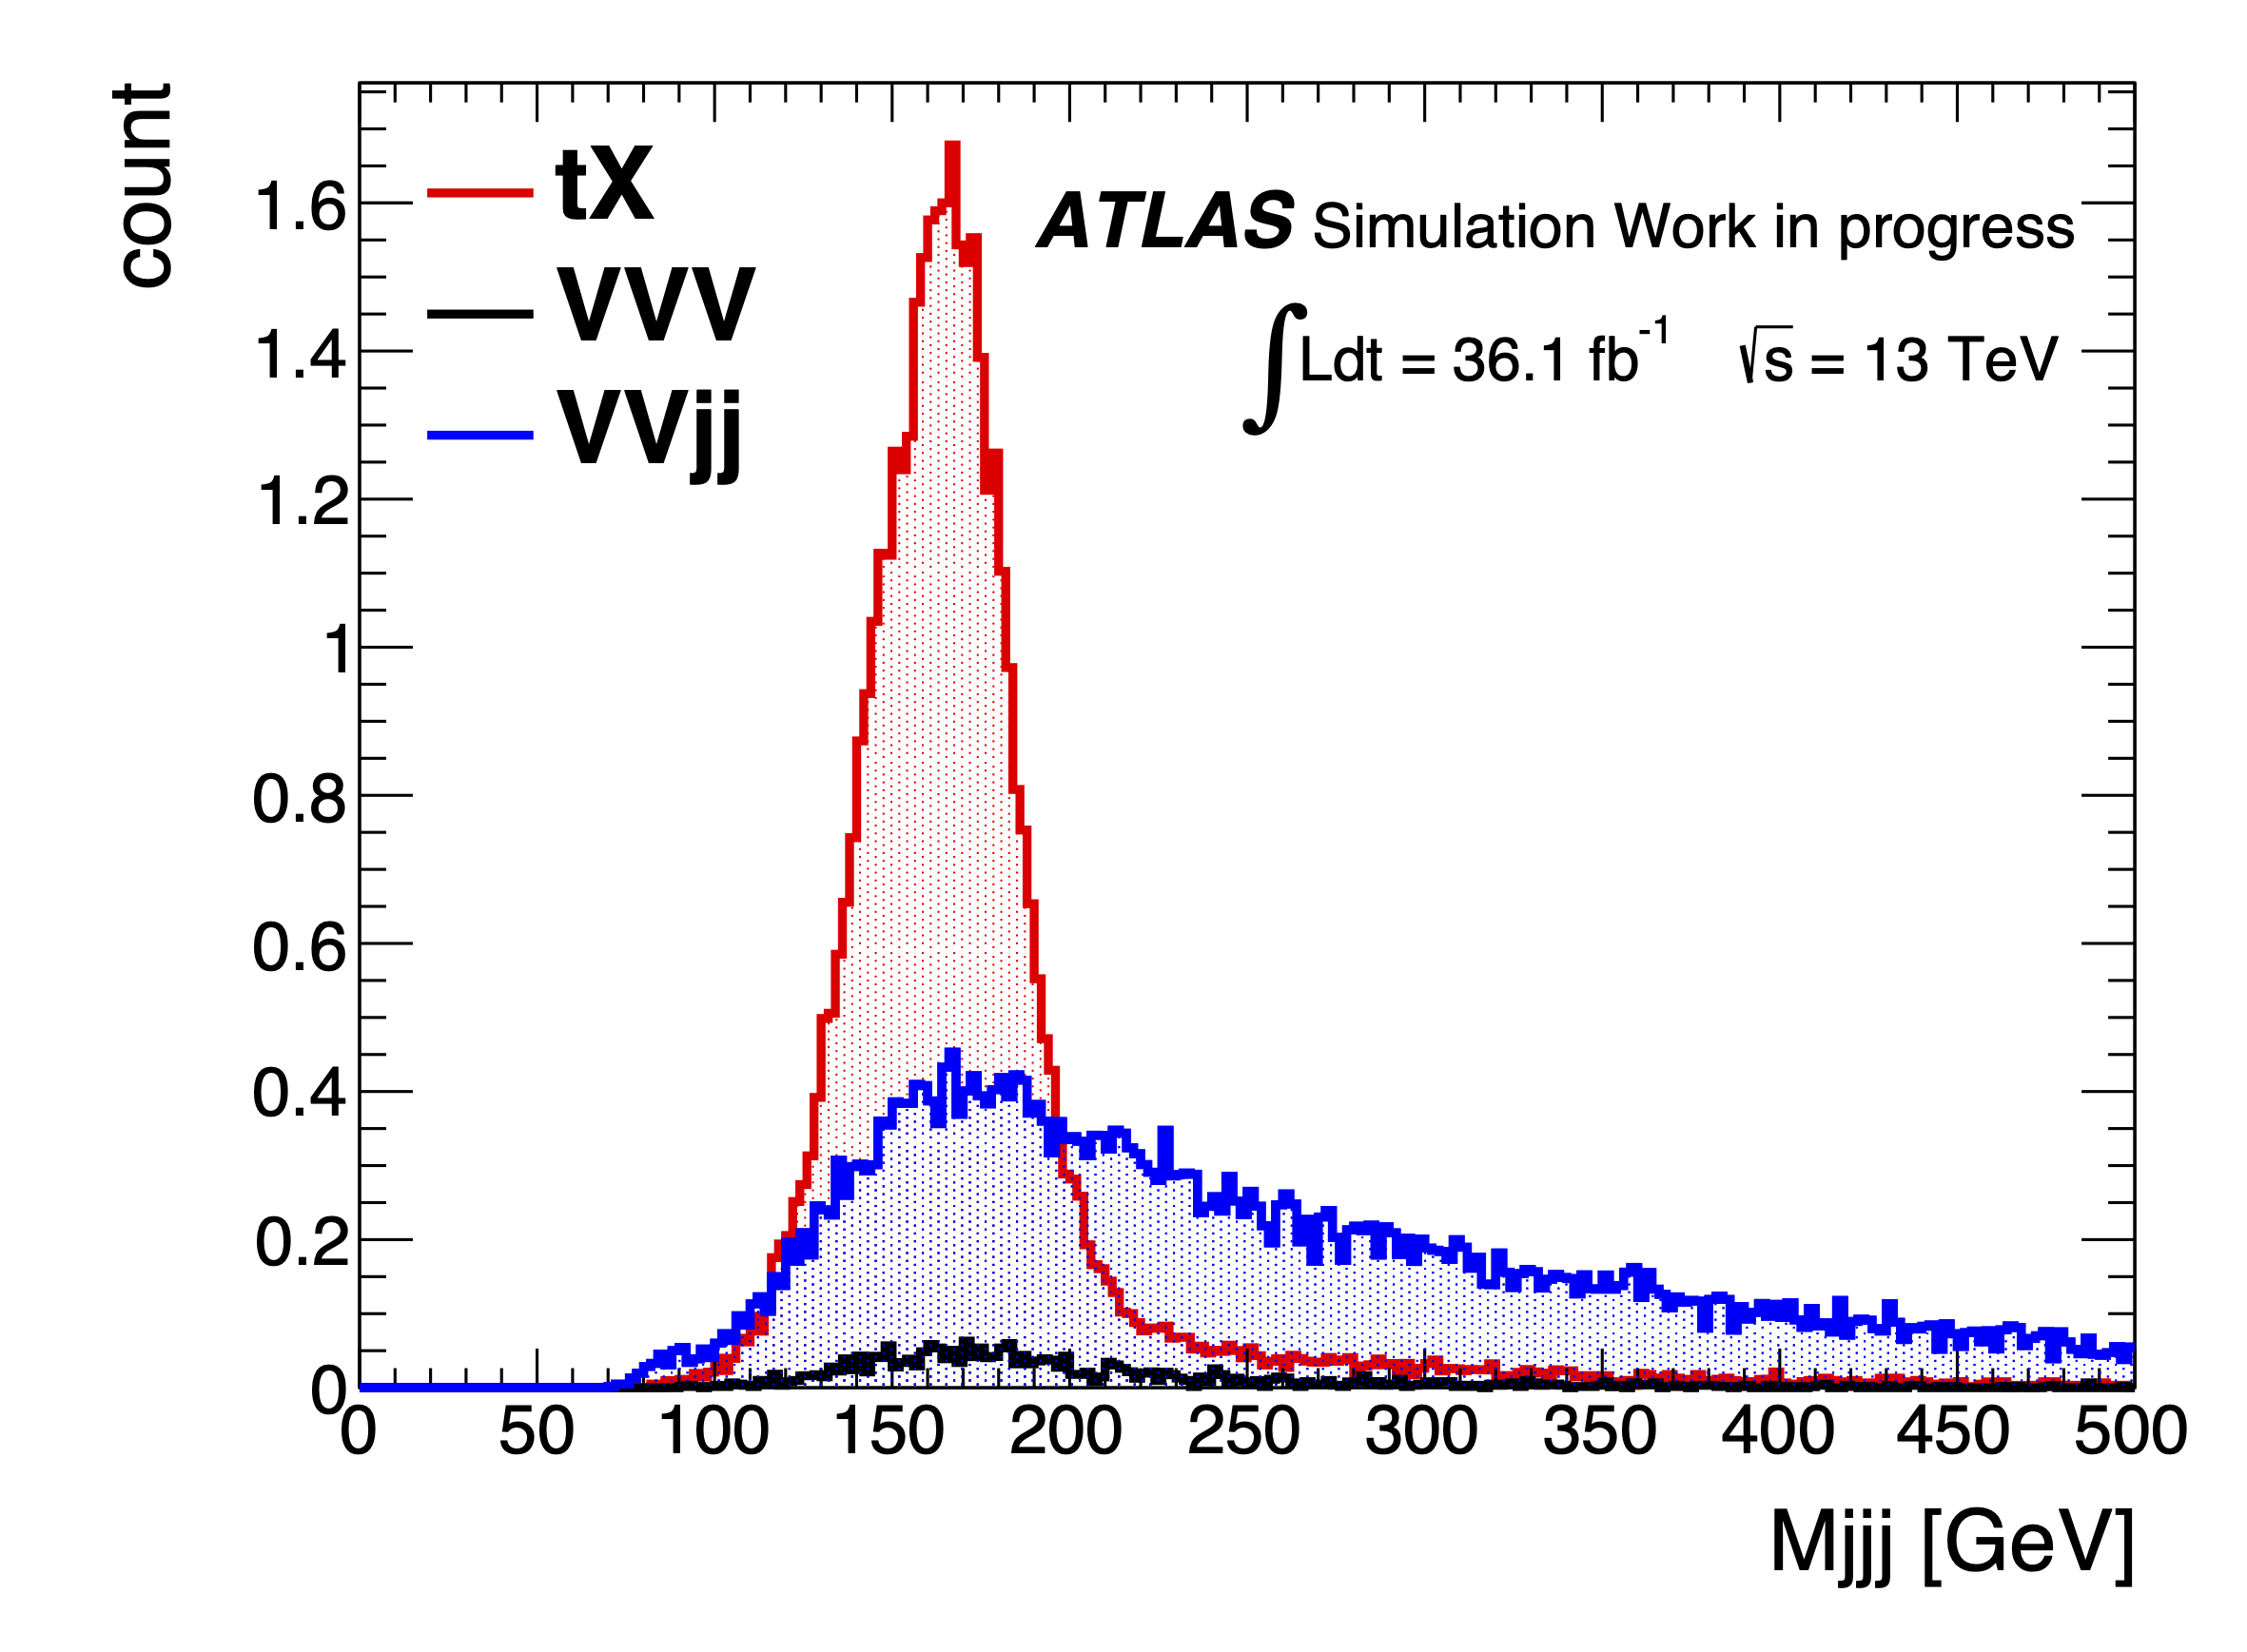
\includegraphics[width=0.45\textwidth]{figures/2lep/topMass/WZjjtopMasspeak}
%      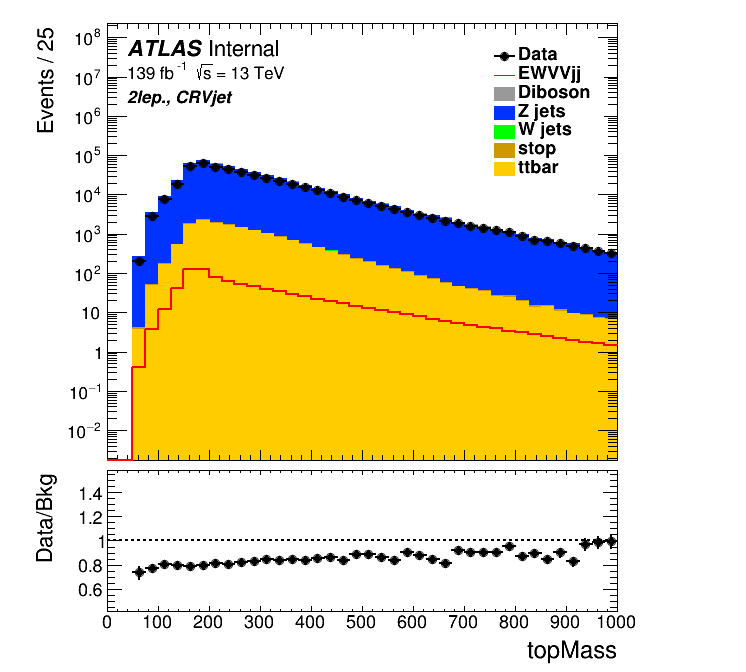
\includegraphics[width=0.45\textwidth]{figures/2lep/dataMC/C_0ptag2pjet_0ptv_CRVjet_topMass_Log}
%       \caption{ Mass of 3 jets in the 2-lepton channel CRVjet.}
%        \label{fig:2leptopMass}
%    \end{center}
%\end{figure}

%Control regions
%There are control regions (CR) are defined to constrain the normalization of the backgrounds. The CRs for the $Z$+jets, $W$+jets, and $t\bar{t}$ events are defined here.
%V+jets CR
%For the merged CRs, the V+jets CRs are defined for the events failing the 80$\%$ WP of the boson tagger. Resolved CRs are defined with using the mass sideband. It is defined with the same event selection as the resolved SR but outside the mass window, which is $50<m_{i i}<64 \mathrm{GeV}$, or $m_{i i}>106 \mathrm{GeV}$.
%top CR
%Top CR is defined only for 1-lepton channel, by requiring at least one b-tagged instead of b-veto. This %Top CR is used for constraining the normalization of the $t\bar{t}$ control region. 

\section{Summary of the event selections}
The summary of the whole event selection applied to the 2-lepton channel is shown here in the Table~\ref{tab:2lep_merged},\ref{tab:2lep_resolved}.
The summaries of the selections applied in each channel are shown here in tables.
%\ref{tab:0lep_merged}-\ref{tab:0lep_resolved}
%\ref{tab:1lep_merged}-\ref{tab:1lep_resolved}
%\ref{tab:2lep_merged}-\ref{tab:2lep_resolved}

%%% 2-leptons channel
\begin{table}[ht!]
\small
\label{tab:2lep_merged}
\begin{center}
\resizebox{\textwidth}{!}{
\begin{tabular}{|l|l|c|c|c|}
\hline
\multicolumn{2}{|l|}{\multirow{2}{*}{Selection}} & \multicolumn{2}{c|}{SR}  &  $Z$ CR \\
\cline{3-5}
\multicolumn{2}{|l|}{} & HP & LP & incl \\
\hline
\multirow{6}{*}{$Z \to \ell\ell$}  &  Number of Loose leptons & \multicolumn{3}{c|}{2} \\
\cline{2-5}
                          & Same flavor &  \multicolumn{3}{c|}{yes} \\
\cline{2-5}
                          & Leading lepton \pt  & \multicolumn{3}{c|}{$>27\,\GeV$} \\
\cline{2-5}
                          & Subleading lepton \pt  & \multicolumn{3}{c|}{$>27\,\GeV$} \\
\cline{2-5}
                          & \multirow{2}{*}{dilepton invariant mass} & \multicolumn{3}{c|}{$ 83 < m_{ee} < 99 \gev$} \\
                          &  & \multicolumn{3}{c|}{$-0.01170\ptll+85.63 < m_{\mu\mu} < 0.01850\ptll+94.00 \gev$} \\
\cline{2-5}
                          & Opposite sign &  \multicolumn{3}{c|}{For $\mu\mu$ channel only} \\
\hline
\multirow{3}{*}{VBS jets candidates} & Leading Tag jet \pt & \multicolumn{3}{c|}{ $>30\,\GeV$ } \\
\cline{2-5}
                          & Subleading Tag jet \pt & \multicolumn{3}{c|}{ $>30\,\GeV$ }\\
\cline{2-5}
                          & $m_{jj}$ & \multicolumn{3}{c|}{ $> 400 \GeV$ } \\
\hline
\multirow{2}{*}{$W/Z \to J$} & Num of large-R jets & \multicolumn{3}{c|}{$\geq 1$} \\
\cline{2-5}
& 3-Var Tagger & pass50WP & pass80WP \&\& !pass50WP & fail80WP \\
\hline
\end{tabular}
}
\end{center}
\caption{A summary of regions event selection for 2-lepton channel in the merged regime.}
\end{table}

\begin{table}[ht!]
\small
\label{tab:2lep_resolved}
\begin{center}
\resizebox{\textwidth}{!}{
\begin{tabular}{|l|l|c|c|}
\hline
\multicolumn{2}{|l|}{Selection} & SR  & $Z$ CR \\
\hline
\multirow{6}{*}{$Z \to \ell\ell$}  &  Number of Loose leptons & \multicolumn{2}{c|}{2} \\
\cline{2-4}
                          & Same flavor &  \multicolumn{2}{c|}{yes} \\
\cline{2-4}
                          & Leading lepton \pt  & \multicolumn{2}{c|}{$>27\,\GeV$} \\
\cline{2-4}
                          & Subleading lepton \pt  & \multicolumn{2}{c|}{$>27\,\GeV$} \\
\cline{2-4}
                          & \multirow{2}{*}{dilepton invariant mass} & \multicolumn{2}{c|}{$ 83 < m_{ee} < 99 \gev$} \\
                          & & \multicolumn{2}{c|}{$-0.01170\ptll+85.63 < m_{\mu\mu} < 0.01850\ptll+94.00 \gev$} \\
\cline{2-4}
                          & Opposite sign &  \multicolumn{2}{c|}{For $\mu\mu$ channel only} \\
\hline
\multirow{3}{*}{VBS jets candidates} & Leading Tag jet \pt & \multicolumn{2}{c|}{ $>30\,\GeV$ } \\\cline{2-4}
                          & Subleading Tag jet \pt & \multicolumn{2}{c|}{ $>30\,\GeV$ }\\
\cline{2-4}
                          & $m_{jj}$ & \multicolumn{2}{c|}{ $> 400 \GeV$ } \\
\hline
\multirow{4}{*}{$W/Z \to jj$} & Num of signal small-R jets & \multicolumn{2}{c|}{2} \\
\cline{2-4}
              & Leading signal jet \pt & \multicolumn{2}{c|}{ $>40\,\GeV$ }\\
\cline{2-4}
              & Subleading signal jet \pt & \multicolumn{2}{c|}{ $>20\,\GeV$ }\\
\cline{2-4}
              &$Z \to q\bar{q}$ and $W \to q\bar{q}$     &   $64 < m_{jj} < 106 \gev$ & $50<m_{jj}<64 \,GeV$ or $m_{jj}>106$ \\
\hline
VBS enhancing & $m_{jjj}$ & \multicolumn{2}{c|}{ $>220$~GeV} \\
\hline
\end{tabular}
}
\end{center}
\caption{A summary of regions event selection for 2-lepton channel in the resolved regime.}
\end{table}

\section{Event selection cutflow}
The cutflow of the event selection in three SRs (HPSR, LPSR, Resolved SR) is shown in Table~\ref{tab:2lep_HPSR},\ref{tab:2lep_LPSR},\ref{tab:2lep_ResolvedSR}. After applying all event selection described here, the signal over background ratio is increased, yet still small, which is about 3~\% in HPSR.

%%% HPSR
\begin{table}[ht!]
\small
\begin{center}
\resizebox{\textwidth}{!}{
 \begin{tabular}{ r ||  r  r  r  r  r  r  r  r  r  || r r r r r |}
 \ensuremath{\sqrt{s}=13 TeV}, \ensuremath{\mathcal{L}=139 fb^{-1}}  & W & WZ & WW & Z & ZZ & stopWtDilep & stops & stopt & ttbar & S & B & S/B & \ensuremath{S/\sqrt{B}}\tabularnewline
 \hline
All & 768630 & 118757 & 7549.85 & 2.69014e+07 & 75904.3 & 219335 & 1566.79 & 30086.3 & 3.4463e+06 & 8530.6 &3.15695e+07&0.00027 & 1.5\tabularnewline \hline
passCommon & 8949.67 & 73105.4 & 138.511 & 1.59613e+07 & 48170 & 22208.8 & 61.7359 & 1002.7 & 361153 & 3577.38&1.64761e+07&0.00021 & 0.88\tabularnewline \hline
TwoTagMerJets & 5430.67 & 41182 & 83.2249 & 9.38413e+06 & 24924.9 & 14016.8 & 33.1233 & 711.353 & 243694 & 2890.74&9.7142e+06&0.00029 & 0.92\tabularnewline \hline
PtTagMerJet1 & 4846.86 & 39715 & 80.198 & 7.66047e+06 & 23830.9 & 13522.8 & 31.7876 & 687.684 & 240045 & 2881.49 &7.98323e+06&0.00036 & 1.01\tabularnewline \hline
PtTagMerJet2 & 2692.05 & 26366.4 & 51.0517 & 3.74324e+06 & 14613 & 8652.04 & 19.427 & 455.492 & 180641 & 2527.77 &3.97673e+06&0.00063 & 1.26\tabularnewline \hline
AtLeastOneFatJet & 73.9896 & 1355.28 & 2.49747 & 54043.4 & 401.963 & 194.503 & 0.683082 & 9.52178 & 4071.51 & 190.792 &60153.4&0.0031 & 0.77\tabularnewline \hline
PtFatJet200 & 73.9896 & 1355.28 & 2.49747 & 54043.4 & 401.963 & 194.503 & 0.683082 & 9.52178 & 4071.51 & 190.792 &60153.4&0.0031 & 0.77\tabularnewline \hline
EtaFatJet2p0 & 73.9896 & 1355.28 & 2.49747 & 54043.4 & 401.963 & 194.503 & 0.683082 & 9.52178 & 4071.51 & 190.792 &60153.4&0.0031 & 0.77\tabularnewline \hline
dRL-eptonFatjet & 65.6967 & 1241.31 & 2.08247 & 50386.7 & 372.277 & 176.007 & 0.617677 & 8.85472 & 3270.23 & 177.47 &55523.8&0.0031 & 0.75\tabularnewline \hline
MFatJetLow & 26.3573 & 593.162 & 1.36814 & 17874.7 & 176.377 & 57.5099 & 0.147335 & 3.37462 & 1340.61 & 120.588 &20073.6&0.0060 & 0.85\tabularnewline \hline
SFLeptons & 8.29704 & 592.425 & 0.528064 & 17868.5 & 176.306 & 19.6953 & 0.0648612 & 1.36886 & 425.456 & 120.184 &19092.6&0.0062 & 0.86\tabularnewline \hline
MFatJet50 & 3.97632 & 321.546 & 0.150938 & 8269.29 & 98.0685 & 9.3015 & 0.0648612 & 0.426969 & 201.394 & 77.5594 &8904.22&0.0087 & 0.82\tabularnewline \hline
D2FatJet50 & 1.6553 & 164.963 & 0.150938 & 3032.68 & 52.9234 & 5.01844 & 0.0207499 & 0.246388 & 81.719 & 50.0044 & 3339.37&0.014 & 0.86\tabularnewline \hline
NTrkFatJet50 & 1.24764 & 114.689 & 0.150938 & 1527.16 & 36.5107 & 2.48592 & 0.0207499 & 0.213116 & 41.1061 & 40.9103 &1723.59&0.023 & 0.98\tabularnewline \hline
WZFatJet50 & 0.655411 & 112.269 & 0.150938 & 1469.7 & 35.6488 & 2.48592 & 0.0207499 & 0.213116 & 39.669 & 40.1491 &1660.82&0.024 & 0.98\tabularnewline \hline
MTagMerJets400 & 0.608311 & 89.745 & 0.150938 & 1247.25 & 27.2269 & 2.34095 & 0.0207499 & 0.0789171 & 33.3017 & 37.6674 &1400.73&0.026 & 1.00\tabularnewline \hline
\end{tabular}
}
\caption{Cutflow table for HPSR region in 2-lepton channel}
\label{tab:2lep_HPSR}
\end{center}
\end{table}

%%% LPSR
\begin{table}[ht!]
\small
\begin{center}
\resizebox{\textwidth}{!}{
 \begin{tabular}{ r ||  r  r  r  r  r  r  r  r  r  || r r r r r |}
 \ensuremath{\sqrt{s}=13 TeV}, \ensuremath{\mathcal{L}=139 fb^{-1}}  & W & WZ & WW & Z & ZZ & stopWtDilep & stops & stopt & ttbar &  S & B & S/B & \ensuremath{S/\sqrt{B}}\tabularnewline
 \hline
All & 768630 & 118757 & 7549.85 & 2.69014e+07 & 75904.3 & 219335 & 1566.79 & 30086.3 & 3.4463e+06 & 8530.6&3.15695e+07&0.00027 & 1.51\tabularnewline \hline
FailMergedSR50 & 768630 & 118667 & 7549.7 & 2.69001e+07 & 75877.1 & 219333 & 1566.77 & 30086.3 & 3.44627e+06 & 8492.93&3.15681e+07&0.00026 & 1.51\tabularnewline \hline
Trigger & 562963 & 108010 & 5681.35 & 2.40927e+07 & 69318 & 195862 & 1133.62 & 21873.2 & 3.02893e+06 & 7222.22 &2.80865e+07&0.00025 & 1.36\tabularnewline \hline
BothLepPt & 67751.3 & 90649.8 & 1147.71 & 2.07619e+07 & 59529.4 & 156592 & 304.094 & 4763.36 & 2.38282e+06 & 4798.78 &2.35255e+07&0.00020 & 0.98\tabularnewline \hline
LeadLepPt & 67452.8 & 90574.8 & 1141.41 & 2.0715e+07 & 59477 & 156269 & 301.881 & 4729.08 & 2.37606e+06 & 4792.64 &2.3471e+07&0.00020 & 0.98\tabularnewline \hline
MuonEtaLt2p5 & 66379 & 89424.2 & 1118.34 & 2.04089e+07 & 58762.6 & 155201 & 291.395 & 4617.26 & 2.3588e+06 & 4734.01 &2.31435e+07&0.00020 & 0.98\tabularnewline \hline
OSMuons & 65152 & 89398.7 & 1101.67 & 2.04087e+07 & 58761 & 155164 & 263.104 & 4354.02 & 2.35796e+06 & 4696.69 &2.31409e+07&0.00020 & 0.97\tabularnewline \hline
Mll & 8949.06 & 73015.6 & 138.36 & 1.596e+07 & 48142.8 & 22206.4 & 61.7151 & 1002.62 & 361120 & 3539.71 &1.64747e+07&0.00021 & 0.87\tabularnewline \hline
TwoTagMerJets & 5430.07 & 41092.3 & 83.0739 & 9.38288e+06 & 24897.7 & 14014.5 & 33.1025 & 711.274 & 243660 & 2853.07&9.7128e+06&0.00029 & 0.91\tabularnewline \hline
PtTagMerJet1 & 4846.25 & 39625.3 & 80.047 & 7.65922e+06 & 23803.7 & 13520.5 & 31.7668 & 687.605 & 240012  & 2843.82&7.98183e+06&0.00035 & 1.00\tabularnewline \hline
PtTagMerJet2 & 2691.44 & 26276.6 & 50.9008 & 3.74199e+06 & 14585.8 & 8649.7 & 19.4063 & 455.413 & 180607  & 2490.1&3.97533e+06&0.00062 & 1.24\tabularnewline \hline
AtLeastOneFatJet & 73.3813 & 1265.54 & 2.34653 & 52796.2 & 374.736 & 192.162 & 0.662332 & 9.44287 & 4038.21 & 153.125&58752.7&0.0026 & 0.63\tabularnewline \hline
PtFatJet200 & 73.3813 & 1265.54 & 2.34653 & 52796.2 & 374.736 & 192.162 & 0.662332 & 9.44287 & 4038.21  & 153.125&58752.7&0.0026 & 0.63\tabularnewline \hline
EtaFatJet2p0 & 73.3813 & 1265.54 & 2.34653 & 52796.2 & 374.736 & 192.162 & 0.662332 & 9.44287 & 4038.21  & 153.125&58752.7&0.0026 & 0.63\tabularnewline \hline
dRLeptonFatjet & 65.0884 & 1151.57 & 1.93153 & 49139.4 & 345.05 & 173.666 & 0.596927 & 8.7758 & 3236.93  & 139.803&54123&0.0025 & 0.60\tabularnewline \hline
MFatJetLow & 25.749 & 503.417 & 1.2172 & 16627.4 & 149.15 & 55.1689 & 0.126585 & 3.29571 & 1307.31 & 82.921 &18672.9&0.0044 & 0.60\tabularnewline \hline
SFLeptons & 7.68872 & 502.68 & 0.377126 & 16621.2 & 149.079 & 17.3543 & 0.0441112 & 1.28994 & 392.155 & 82.5162 &17691.9&0.0046 & 0.62\tabularnewline \hline
MFatJet80 & 4.50972 & 305.264 & 0.0531649 & 9708.43 & 92.5334 & 9.79512 & 0.0441112 & 0.8637 & 230.263 & 53.3019 &10351.8&0.0051& 0.52\tabularnewline \hline
D2FatJet80 & 3.0742 & 220.826 & 0 & 6606.32 & 67.506 & 8.12447 & 0 & 0.652429 & 167.653 & 40.3886 &7074.16&0.0057 & 0.48\tabularnewline \hline
NTrkFatJet80 & 1.80329 & 175.492 & 0 & 4548.12 & 53.5843 & 4.93659 & 0 & 0.58877 & 106.823 & 36.0306 &4891.35&0.0073 & 0.51\tabularnewline \hline
WZFatJet80 & 1.80329 & 170.838 & 0 & 4389.69 & 52.4945 & 4.55232 & 0 & 0.58877 & 103.266 & 35.429 &4723.23&0.0075 & 0.51\tabularnewline \hline
MTagMerJets400 & 1.67793 & 123.578 & 0 & 3541.1 & 35.3674 & 3.94765 & 0 & 0.454571 & 80.232 & 30.8227 &3786.36&0.0081 & 0.50\tabularnewline \hline
\end{tabular}
}
\caption{Cutflow table for LPSR region in 2-lepton channel}
\label{tab:2lep_LPSR}
\end{center}
\end{table}

%% Resolved SR
\begin{table}[ht!]
\small
\begin{center}
\resizebox{\textwidth}{!}{
 %\begin{tabular}{ r ||  r  r  r  r  r  r  r  r  r  r || r r r r r |}
 \begin{tabular}{ r ||  r  r  r  r  r  r  r  r  r  || r r r r r |}
 \ensuremath{\sqrt{s}=13 TeV}, \ensuremath{\mathcal{L}=139 fb^{-1}}  & W & WZ & WW & Z & ZZ & stopWtDilep & stops & stopt & ttbar & S  & B & S/B & \ensuremath{S/\sqrt{B}}\tabularnewline
 \hline
All & 768630 & 118757 & 7549.85 & 2.69014e+07 & 75904.3 & 219335 & 1566.79 & 30086.3 & 3.4463e+06 & 8530.6 &3.15695e+07&0.00027 & 1.51\tabularnewline \hline
FailMergedSR50 & 768630 & 118667 & 7549.7 & 2.69001e+07 & 75877.1 & 219333 & 1566.77 & 30086.3 & 3.44627e+06 & 8492.93&3.15681e+07&0.00026 & 1.51\tabularnewline \hline
FailMergedSR80 & 768628 & 118544 & 7549.7 & 2.68966e+07 & 75841.7 & 219329 & 1566.77 & 30085.8 & 3.44619e+06 & 8462.11&3.15643e+07&0.00026 & 1.50\tabularnewline \hline
Trigger & 562961 & 107887 & 5681.35 & 2.40892e+07 & 69282.7 & 195858 & 1133.62 & 21872.7 & 3.02885e+06 & 7191.4 &2.80827e+07&0.00025 & 1.35\tabularnewline \hline
BothLepPt & 67749.6 & 90526.2 & 1147.71 & 2.07584e+07 & 59494 & 156588 & 304.094 & 4762.91 & 2.38274e+06 & 4767.96 &2.35217e+07&0.00020 & 0.98\tabularnewline \hline
LeadLepPt & 67451.1 & 90451.2 & 1141.41 & 2.07115e+07 & 59441.7 & 156265 & 301.881 & 4728.63 & 2.37598e+06 & 4761.82 &2.34672e+07&0.00020 & 0.98\tabularnewline \hline
MuonEtaLt2p5 & 66377.3 & 89300.6 & 1118.34 & 2.04053e+07 & 58727.3 & 155197 & 291.395 & 4616.81 & 2.35872e+06 & 4703.18 &2.31397e+07&0.00020 & 0.97\tabularnewline \hline
OSMuons & 65150.4 & 89275.1 & 1101.67 & 2.04052e+07 & 58725.7 & 155160 & 263.104 & 4353.56 & 2.35788e+06 & 4665.87 &2.31371e+07&0.00020 & 0.97\tabularnewline \hline
Mll & 8947.38 & 72892.1 & 138.36 & 1.59565e+07 & 48107.4 & 22202.5 & 61.7151 & 1002.17 & 361040 & 3508.89 &1.64709e+07&0.00021 & 0.86\tabularnewline \hline
TwoTagResJets & 5428.39 & 40968.7 & 83.0739 & 9.37934e+06 & 24862.3 & 14010.5 & 33.1025 & 710.82 & 243580 & 2822.25&9.70902e+06&0.00029 & 0.90\tabularnewline \hline
PtTagResJet1 & 4844.57 & 39501.7 & 80.047 & 7.65568e+06 & 23768.3 & 13516.5 & 31.7668 & 687.15 & 239932 & 2813 &7.97804e+06&0.00035 & 0.99\tabularnewline \hline
PtTagResJet2 & 2689.76 & 26153.1 & 50.9008 & 3.73845e+06 & 14550.4 & 8645.75 & 19.4063 & 454.958 & 180527 & 2459.28 &3.97154e+06&0.00061 & 1.23\tabularnewline \hline
TwoSigJets & 1224.28 & 15670.2 & 27.3266 & 1.35255e+06 & 7188.69 & 3383.22 & 6.95563 & 193.559 & 97769.1 & 1983.71 &1.47801e+06&0.0013 & 1.63\tabularnewline \hline
PtSignalJet1 & 895.835 & 12934.8 & 23.2614 & 908980 & 5628.78 & 2675.5 & 5.30779 & 148.163 & 83593 & 1796.12 &1.01488e+06&0.0017 & 1.78\tabularnewline \hline
PtSignalJet2 & 895.835 & 12934.8 & 23.2614 & 908980 & 5628.78 & 2675.5 & 5.30779 & 148.163 & 83593 & 1796.12 &1.01488e+06&0.0017 & 1.78\tabularnewline \hline
MVHadResLow & 786.438 & 11881.2 & 21.6767 & 797009 & 5103.81 & 2390.64 & 4.78611 & 135.01 & 75903.6 & 1690.66&893237&0.0018 & 1.78\tabularnewline \hline
SFLeptons & 238.494 & 11869.8 & 8.04294 & 796752 & 5102.21 & 738.483 & 1.51008 & 43.6911 & 23211.2 & 1673.08&837966&0.0019 & 1.82\tabularnewline \hline
MVHadRes & 82.6204 & 3972.79 & 2.81781 & 251182 & 1838.78 & 204.164 & 0.436533 & 12.379 & 6566.27 & 782.652&263862&0.0029 & 1.52\tabularnewline \hline
MTagResJets400 & 36.9849 & 1922.17 & 1.59711 & 139844 & 814.46 & 100.109 & 0.263526 & 9.07562 & 3048.05 & 581.914&145777&0.0039 & 1.52\tabularnewline \hline
passMjjjRes & 15.7732 & 479.481 & 0.603948 & 37458.8 & 189.746 & 32.6127 & 0.0863601 & 3.17091 & 888.228 & 177.763&39068.5&0.0045 & 0.89\tabularnewline \hline
\end{tabular}
}
\caption{Cutflow table for Resolved SR region in 2-lepton channel}
\label{tab:2lep_ResolvedSR}
\end{center}
\end{table}




